%==============================================================================
% Learning to Spread Edges: Reinforcement-Learning Construction of
% Spatially-Coupled LDPC Codes  --  IEEE Transactions on Communications draft
%
% Build:  pdflatex main && bibtex main && pdflatex main && pdflatex main
%
%------------------------------------------------------------------------------
% OUTSTANDING TODOs (search the source for "TODO:" -- each maps to an experiment
% or fact still to be completed; all appear in-text as \textcolor{red}{[TODO: ...]}):
%
%   TODO-1/2/3 (PEXIT-*): RESOLVED.  PEXIT threshold analysis is run and folded
%                     in (Sec. IV / Table tab:pexit).  Correctness gate passes
%                     ((3,6)=1.105 dB vs 1.10), within-cell construction-invariant
%                     (0.013-0.042 dB spread, threshold saturation), cross-rate
%                     Spearman 0.90-1.00, PEXIT-reward null result.
%   TODO-5 (author): real author names, affiliation, e-mail, funding/ack.
%==============================================================================

\documentclass[journal]{IEEEtran}

\usepackage{amsmath,amssymb,amsfonts}
\usepackage{algorithmic}
\usepackage{graphicx}
\usepackage{textcomp}
\usepackage{xcolor}
\usepackage{booktabs}
\usepackage{array}
\usepackage{multirow}
\usepackage{url}
\usepackage[colorlinks=true,allcolors=blue]{hyperref}

% A visible TODO macro so the human can grep / eyeball every pending item.
\newcommand{\TODO}[1]{\textcolor{red}{[TODO: #1]}}

\graphicspath{{figs/}}

\begin{document}

\title{Learning to Spread Edges: Reinforcement-Learning\\
Construction of Spatially-Coupled LDPC Codes}

% TODO-5: author block placeholder
\author{Yye~\textit{et~al.}%
\thanks{\TODO{author names, affiliation, e-mail, and funding acknowledgement.}
Manuscript drafted June 2026.}}

\markboth{IEEE Transactions on Communications (Draft)}%
{Yye \MakeLowercase{\textit{et al.}}: Learning to Spread Edges}

\maketitle

%==============================================================================
\begin{abstract}
%==============================================================================
Spatially-coupled low-density parity-check (SC-LDPC) codes are built from a
component protograph by \emph{edge spreading}: each systematic base edge is
assigned to one of $w{+}1$ coupling components $B_0,\dots,B_w$. In standard
5G-NR-based constructions this assignment is left to a random number generator,
yet we measure that this single random choice changes the frame-error rate
(FER) at a fixed operating point by roughly $7\times$. We make four
contributions. \textbf{(C1)} We show that edge spreading is a high-leverage but
routinely randomized design freedom: optimizing it alone lowers FER by
$5$--$11\times$ and \emph{eliminates the error floor}; the gain holds across
code rates $0.5$--$0.9$, with a waterfall-threshold gain of $0.12$--$0.92$\,dB
that is largest ($\sim\!0.9$\,dB) at $R\!\approx\!0.6$ and shrinks monotonically
toward high rate. \textbf{(C2)} We cast edge spreading as a Markov decision
process (MDP) and optimize it end-to-end with policy gradient (REINFORCE),
using the FER of the real encode/channel/window-decode chain as the reward. The
learned $8$-parameter feature policy removes the dominant population of
$4$-cycles (girth $4\!\to\!6$, $n_4\!\approx\!930\!\to\!0$); we prove an exact,
bit-exact-validated combinatorial lemma characterizing the $4$-cycle count under
edge spreading---$n_4=\sum_{\mathrm{keys}} Z\,\binom{m}{2}$ over (check-block-row,
column-pair, shift-difference) keys---which explains why naive constructions
carry $\approx\!930$ $4$-cycles, why no simple balance rule removes them (the
shift-differences are fixed by the 5G-NR circulants, not by the construction),
and hence why a search-based construction is needed. A validated protograph EXIT
(PEXIT) analysis (correctness gate within $0.005$\,dB of the $(3,6)$ textbook
threshold) explains the rate dependence of the waterfall gain via threshold
saturation: the asymptotic threshold is construction-invariant within a rate
cell ($\le0.04$\,dB spread) yet tracks the Monte-Carlo waterfall across rates
(Spearman $0.90$--$1.00$). \textbf{(C3)} We give a deployable criterion for
\emph{when} reinforcement learning helps: its sample-efficiency advantage over
blind random search grows monotonically with per-evaluation cost and search-space
size $(w{+}1)^E$---RL wins $13/15$ long-code cells (advantage growing with $w$),
while under a cheap surrogate it merely ties. \textbf{(C4)} The feature policy
transfers \emph{zero-shot} to new lifting sizes and rates, a deployment property
that random search and the cross-entropy method (CEM) cannot offer.
\end{abstract}

\begin{IEEEkeywords}
Spatially-coupled LDPC codes, edge spreading, code construction,
reinforcement learning, policy gradient, 5G NR, error floor,
threshold saturation, quasi-cyclic codes.
\end{IEEEkeywords}

%==============================================================================
\section{Introduction}\label{sec:intro}
%==============================================================================
\IEEEPARstart{S}{patially}-coupled LDPC (SC-LDPC) codes couple a chain of
otherwise independent LDPC component codes along a spatial dimension; under
belief-propagation (BP) decoding of a terminated chain, their threshold
\emph{saturates} to the maximum-a-posteriori (MAP) threshold of the underlying
component ensemble~\cite{kudekar2011threshold,felstrom1999ldpcc}. This makes
SC-LDPC a strong candidate for low-latency, streaming, and 6G channel coding,
and the 5G-NR quasi-cyclic (QC) base graphs of 3GPP TS~38.212~\cite{3gpp38212}
provide a standardized, efficiently encodable starting point.

An SC-LDPC code is obtained from a component protograph by \emph{edge
spreading}: writing the component base matrix as
$B = B_0 + B_1 + \dots + B_w$, each base edge is assigned to exactly one
component $B_a$, and the variable position $t$ connects through $B_a$ to check
position $t{+}a$~\cite{mitchell2015scldpc}. Different edge spreadings are known
to affect \emph{both} the iterative BP performance and the distance/cycle
properties of the resulting code~\cite{mitchell2015scldpc}. Yet in practice---and
in the original version of the open-source pipeline used here---this assignment
is simply drawn from a random number generator. The single line
\texttt{rng.integers(0,w+1,size=E)} is, in effect, an unexamined design
decision.

How much does that decision matter? On a fixed channel realization (i.e.\
using common random numbers so that only the construction changes), we measure
the FER of $14$ \emph{random} edge spreadings at one operating point and observe
a spread of $0.106$ to $0.725$---about a $7\times$ swing in FER from this one
random choice alone (Section~\ref{sec:results-headroom}). The construction
space is enormous: $(w{+}1)^E$ with $E$ systematic base edges, e.g.\ $3^{40}
\approx 10^{19}$ for the deep-dive configuration and as large as $31^{121}$ for
the wide-memory sweeps. Edge spreading is therefore a high-leverage but
routinely randomized construction freedom.

\textbf{Contributions.} We position this work as a finite-length
\emph{coding-engineering} paper in which a learning method is the tool and the
code is the subject. Concretely:
\begin{itemize}
\item \textbf{C1 (the hard result).} Optimizing edge spreading---and nothing
else---lowers FER by $5$--$11\times$ and \emph{eliminates the error floor};
the gain holds over rates $0.5$--$0.9$, with a waterfall-threshold gain of
$0.12$--$0.92$\,dB, largest at $R\!\approx\!0.6$ and shrinking toward high rate
(Sections~\ref{sec:results-c1}, \ref{sec:results-rate}).
\item \textbf{C2 (mechanism and theory).} We cast construction as an MDP and
optimize it end-to-end by policy gradient; the learned $8$-parameter policy
removes the dominant population of $4$-cycles. We prove an exact,
bit-exact-validated combinatorial lemma characterizing the $4$-cycle count
under edge spreading, $n_4=\sum_{\mathrm{keys}} Z\,\binom{m}{2}$ over
(check-block-row, column-pair, shift-difference) keys (Section~\ref{sec:lemma}),
which explains why naive constructions carry $\approx\!930$ $4$-cycles, why no
simple balance rule removes them (the shift-differences are fixed by the 5G-NR
circulants), and hence why search-based construction is needed; and a validated
protograph EXIT (PEXIT) analysis explains the rate dependence of the gain via
threshold saturation---the asymptotic threshold is construction-invariant within
a rate cell yet tracks the Monte-Carlo waterfall across rates (Spearman
$0.90$--$1.00$; Section~\ref{sec:pexit}).
\item \textbf{C3 (a methodological criterion).} The sample-efficiency advantage
of RL over random search/CEM grows monotonically with per-evaluation cost and
search-space size $(w{+}1)^E$: RL wins $13/15$ long-code cells with the
advantage growing in $w$, but ties under a cheap surrogate
(Sections~\ref{sec:results-bigw}, \ref{sec:results-wsweep},
\ref{sec:results-wproxy}). This is a deployable ``when to use RL'' criterion.
\item \textbf{C4 (a deployment property).} The feature policy transfers
zero-shot to new lifting sizes and rates---something random search/CEM, which
produce a code-specific assignment vector, cannot do
(Section~\ref{sec:results-transfer}).
\end{itemize}

The remainder follows the structure: Section~\ref{sec:background} reviews
SC-LDPC and edge spreading; Section~\ref{sec:mdp} casts construction as an MDP;
Section~\ref{sec:pexit} develops the threshold (PEXIT) objective;
Section~\ref{sec:lemma} states the combinatorial lemma;
Section~\ref{sec:setup} describes baselines and setup;
Section~\ref{sec:results} reports results;
Section~\ref{sec:discussion} discusses limitations, including a scoped negative
result on the error floor; and Section~\ref{sec:conclusion} concludes.

\subsection{Related Work and Distinction}\label{sec:related}
We organize prior art along two axes: decoding versus construction, and block
versus spatially-coupled codes.

\emph{RL for LDPC \textbf{decoding}} is mature: RELDEC casts cluster scheduling
as an MDP and learns sequential schedules for 5G-NR LDPC~\cite{habib2023reldec};
our companion line learns sliding-window scheduling for SC-LDPC. In all of these
the code is \emph{given}.

\emph{AI/RL for \textbf{code construction}} exists but not for spatial coupling.
``AI Coding''~\cite{huang2020aicoding} proposes a constructor--evaluator
framework (RL or a genetic algorithm) for \emph{linear block / polar} codes;
a deep-RL/MCTS approach learns PEG-style edge growth for LDPC \emph{block}
codes~\cite{zhang2018ldpcdrl}. Neither targets SC-LDPC nor edge spreading.

\emph{SC-LDPC \textbf{construction}} has been studied with non-learning search:
Mitchell--Lentmaier--Costello define edge spreading and quantify its
effect~\cite{mitchell2015scldpc}; high-rate array-based edge spreading is
designed in~\cite{mitchell2017edgespreading}; greedy elimination of harmful
objects is used in~\cite{battaglioni2019harmful}; the partition matrix is
optimized by exhaustive traversal with pruning
in~\cite{esfahanizadeh2022unified,hareedy2025adaptorregress}, whose authors note
that such discrete optimization ``struggles as more degrees of freedom appear'';
a 6G edge-spreading Raptor-like construction~\cite{ren2024esrl} and an MCMC
sampler~\cite{tanrikulu2025mcmc} are likewise non-RL. After an extensive
literature check, \emph{no published work casts SC-LDPC construction / edge
spreading as an MDP and optimizes it with reinforcement learning}; existing
methods are greedy, exhaustive, graph-theoretic, or MCMC. Our methodological
template is the neural combinatorial optimization framework of
Bello~\textit{et~al.}~\cite{bello2016neural} with the REINFORCE
estimator~\cite{williams1992reinforce}. Table~\ref{tab:distinction} summarizes
the distinction from the closest works.

\begin{table}[t]
\centering
\caption{Distinction From the Closest Works.}
\label{tab:distinction}
\renewcommand{\arraystretch}{1.2}
\setlength{\tabcolsep}{3pt}
\footnotesize
\begin{tabular}{@{}lccc@{}}
\toprule
 & AI Coding & Esfahanizadeh / & \textbf{This work}\\
 & \cite{huang2020aicoding} & Battaglioni & \\
\midrule
Code      & block/polar    & SC-LDPC                 & SC-LDPC\\
Object    & gen./parity    & partition matrix        & \textbf{edge-spread assign}\\
Method    & RL / GA        & greedy/exhaustive/MCMC  & \textbf{policy-gradient MDP}\\
Reward    & dist./thr./BER & asy.\ thr.\ + cycles    & \textbf{end-to-end FER}\\
Transfer  & ---            & no (re-search)          & \textbf{yes (zero-shot)}\\
\bottomrule
\end{tabular}
\end{table}

%==============================================================================
\section{Background}\label{sec:background}
%==============================================================================
\subsection{From Block Codes to a Coupled Chain}
An LDPC block code is defined by a fixed parity-check matrix $H$ (Tanner graph).
An SC-LDPC code couples a chain of LDPC component codes---each described by a
protograph / base matrix $B$ of size $m_b \times n_b$---along the spatial
dimension. First introduced as LDPC convolutional
codes~\cite{felstrom1999ldpcc}, the protograph view was systematized
by~\cite{kudekar2011threshold}.

\subsection{Edge Spreading and the Band-Diagonal Matrix}
Given coupling memory $w$, edge spreading splits $B$ into $w{+}1$ component
matrices,
\begin{equation}
B = B_0 + B_1 + \dots + B_w,
\end{equation}
with each base edge assigned to exactly one component. Staggering the components
along the diagonal yields a band-diagonal coupled parity-check matrix with block
structure
\begin{equation}
H_{\mathrm{SC}}[i,t] = B_{\,i-t}\quad\text{for } 0 \le i-t \le w,
\end{equation}
where $t = 0,\dots,L{-}1$ indexes variable (column) positions and
$i = 0,\dots,L{+}w{-}1$ indexes check (row) positions over a coupling length
$L$. Variable position $t$ thus connects through $B_0,\dots,B_w$ to check
positions $t,\dots,t{+}w$.

\subsection{Termination and Rate Loss}
The $w$ extra check positions at the tail are the \emph{termination}: they
impose stronger constraints at the chain boundaries (lower-degree, more reliable
checks), at the cost of a small rate loss. The coupled rate $R_L$ satisfies
$R_L \to R$ as $L \to \infty$, with rate loss of order $w/L$.

\subsection{Threshold Saturation}\label{sec:thr-sat}
The central theoretical property of SC-LDPC is threshold
saturation~\cite{kudekar2011threshold}: the BP threshold of a terminated
SC-LDPC ensemble saturates to the MAP threshold of its component ensemble.
Termination triggers a \emph{decoding wave} that propagates reliability inward
from the boundaries; this is the mechanism by which suboptimal iterative
decoding is lifted, essentially for free, to near-MAP performance. Sliding-window
decoding~\cite{iyengar2011windowed} exploits the locality of this wave: BP is run
only inside a window of $W$ positions, so latency and storage scale with $W$
rather than $L$. We use $W = w{+}1$ throughout.

\subsection{5G-NR Systematic Edge Spreading}\label{sec:sysedge}
We build SC-LDPC from the 5G-NR QC-LDPC base graphs of 3GPP
TS~38.212~\cite{3gpp38212} (BG1: $46\times68$, $K_b{=}22$; BG2: $42\times52$,
$K_b{=}10$). To preserve the efficiently encodable double-diagonal /
accumulator parity structure of 5G NR, we spread only the \emph{systematic}
base edges (the first $K_b$ columns) across $B_0,\dots,B_w$ and keep the entire
parity part in $B_0$. Each position is then encoded by the standard 5G recursion,
and the coupled $H_{\mathrm{SC}}c=0$ holds exactly. The set of $E$ systematic
base edges is the construction variable; the parity structure and QC lifting
shifts are fixed. Why edge spreading is a natural fit for sequential
optimization: it is an inherently sequential assignment process (each edge in
turn picks a component), its quality is governed by the cycle structure of the
lifted graph, and that structure is highly sensitive to each edge's
assignment---precisely where a policy gradient can climb a structural gradient
while blind search cannot efficiently cover $(w{+}1)^E$.

%==============================================================================
\section{Construction as a Markov Decision Process}\label{sec:mdp}
%==============================================================================
We construct a code edge-by-edge in a fixed row-major order
$e_0,\dots,e_{E-1}$ and cast it as an MDP.

\subsection{State, Action, Reward}
\begin{itemize}
\item \textbf{Episode:} construct one full code (assign all $E$ edges) and
evaluate it end-to-end.
\item \textbf{Time step $t$:} choose a component $a_t \in \{0,\dots,w\}$ for
edge $e_t$.
\item \textbf{State $s_t$:} features of edge $e_t$ under the \emph{current
partial construction}. For each candidate component $a$ we compute the fraction
of edges in the same base \emph{row} already assigned to $a$ (\texttt{row\_frac}),
the same fraction by base \emph{column} (\texttt{col\_frac}), the \emph{global}
load fraction of $a$ (\texttt{glob\_frac}), and binary indicators of whether $a$
is still empty for this row / column (\texttt{row\_empty}, \texttt{col\_empty}).
These running counts make the process a genuinely sequential MDP and let the
policy learn structural rules such as balancing component loads within a row or
column.
\item \textbf{Action $a_t$:} the component index.
\item \textbf{Reward:} intermediate rewards are $0$; at the end of the episode
a terminal reward $R = -\text{FER}$ is given, obtained by placing the
constructed code into the \emph{real} encode~$\to$~BPSK+AWGN~$\to$
sliding-window BP~$\to$ FER chain at the training SNR over a batch of
common-random-number (CRN) frames. The ground truth is used only to score a
constructed code at design time; the learned construction (the assignment
vector) carries no ground truth and is directly deployable, exactly as for any
code design.
\end{itemize}

\subsection{Policy Gradient}
Maximizing $\mathbb{E}[R]$ over the factorized policy
$\pi_\theta(a) = \prod_t \pi(a_t \mid s_t)$ is
REINFORCE~\cite{williams1992reinforce,bello2016neural}:
\begin{equation}
\nabla J = \mathbb{E}\!\left[(R-b)\sum_t \nabla \log \pi(a_t\mid s_t)\right],
\end{equation}
where $b$ is an \emph{in-batch baseline} (the mean of $R$ over the batch). On top
of this we use \emph{common random numbers}: every candidate code in a batch is
scored on the \emph{same} frames, so the advantage $R_i-b$ has very low variance
and the policy learns stably even when each code is scored on only a few frames.
This variance reduction is what makes the method tractable on CPU. We optimize
with Adam (pure NumPy), standardize advantages within a batch, and add an entropy
bonus to encourage exploration. Both policy gradients are verified by finite
differences.

\subsection{Two Policies}\label{sec:policies}
\begin{enumerate}
\item \textbf{Feature policy (primary).} A linear softmax over the per-component
features, with parameters $w{+}1$ component biases plus a handful of shared
weights---\emph{8 numbers in total for $w{=}2$, independent of the code size.}
Hence the learned policy can transfer zero-shot to codes with different
$Z/L/$rate (provided $w$ matches), and it is interpretable.
\item \textbf{Per-edge policy (ablation).} Independent logits per edge
($E\times C$ parameters): maximally expressive but non-transferable, used as a
control for whether a generalizing structure is needed.
\end{enumerate}

\subsection{Algorithmic Notes}
The implementation is pure NumPy with multiprocessing over CPU cores; the masks
(puncturing/termination/transmitted positions) depend only on $L,w,K_b,n_b,Z$
and \emph{not} on the assignment, so all candidate codes can be scored on
bit-identical information and noise (CRN), which the evaluator is tested to
reproduce bit-exactly. The champion of each method is re-tested on an
\emph{independent}, larger frame bank to remove selection noise.

%==============================================================================
\section{A Threshold (PEXIT) Objective}\label{sec:pexit}
%==============================================================================
This section develops a \emph{frame-free}, density-evolution-grounded
predictor that (a) addresses the ``Monte-Carlo only'' concern with a
validated analytic threshold, and (b) \emph{explains} the rate dependence of
the waterfall gain observed in C1 via threshold saturation. We are explicit
about scope: protograph EXIT (PEXIT) is \emph{cheap} and frame-free (the
correctness gate and all five rate cells run in $\approx\!50$\,s, serially),
so it is \emph{not} an expensive objective and is \emph{not} the basis of the
C3 ``expensive evaluation $\Rightarrow$ RL wins'' argument---that argument
stands on its own through the long-code Monte-Carlo of
Sections~\ref{sec:results-bigw}--\ref{sec:results-wproxy}. PEXIT's honest role
is twofold: a validated explanation of \emph{why} the asymptotic threshold
(hence the waterfall) is construction-robust, and a cheap cross-rate predictor
of the Monte-Carlo waterfall ordering.

\subsection{Why Asymptotic Thresholds Are Nearly Construction-Invariant}
By threshold saturation (Section~\ref{sec:thr-sat}), the asymptotic BP threshold
of a good terminated SC-LDPC ensemble approaches the component MAP threshold,
\emph{independently of fine construction detail}. This is precisely why the
asymptotic threshold cannot, on its own, separate two good edge spreadings: the
BP--MAP gap that coupling fills is large at low rate (strong component, many
checks per position) and small at high rate (weak component). Consequently the
\emph{waterfall} construction gain is largest at moderate rate and shrinks toward
high rate---exactly the trend measured in Section~\ref{sec:results-rate}. What
\emph{does} separate finite-length constructions is the finite-length PEXIT
recursion including the termination boundary, together with the cycle structure.

\subsection{Protograph EXIT for the Coupled Graph}
We adopt protograph EXIT (PEXIT)~\cite{liva2007pexit} over the band-diagonal
protograph defined by the assignment (components $B_0,\dots,B_w$, coupling length
$L$, and the termination boundary), using the BIAWGN $J/J^{-1}$ mutual-information
transfer functions and the finite-length protograph analysis
of~\cite{stinner2014finitelength}. The recursion returns (i) the $E_b/N_0$
threshold required for convergence and (ii) a finite-length PEXIT BER proxy.
The same pipeline can plug this in as a reward via
$R = -\text{threshold}_{E_b/N_0}$, reusing the REINFORCE machinery unchanged
and replacing the Monte-Carlo evaluator with a PEXIT evaluator; we report below
that this reward is essentially flat within a rate cell (threshold saturation),
so the PEXIT-reward loop is auto-disabled---a null result that is itself part
of the theory.

\subsection{Honest Scope}
We do \emph{not} claim that a PEXIT threshold strongly discriminates
constructions \emph{within a rate cell}---threshold saturation makes the
thresholds of good constructions converge, which is itself the theory to be
told (and which we confirm numerically below: the within-cell spread over
round-robin plus random edge spreadings is only $0.013$--$0.042$\,dB). PEXIT is
moreover \emph{cheap and frame-free}---the entire analysis (correctness gate
plus all five rate cells) runs in $\approx\!50$\,s serially---so it is
\emph{not} the expensive principled objective and, by the same token, is
\emph{not} a useful within-cell reward (there is essentially nothing to
optimize once the construction is $4$-cycle-free; see the null result below).
Its two legitimate roles are: \emph{(i)} an \emph{explanation}---a validated
density-evolution account of why the asymptotic threshold, and hence the
Monte-Carlo waterfall, is construction-robust while the finite-length floor is
not; and \emph{(ii)} a cheap \emph{cross-rate predictor} of the waterfall
ordering. The discriminating quantity for the finite-length \emph{floor}
remains the cycle/trapping-set structure, not the threshold.

\subsection{Validation}\label{sec:pexit-val}
We implement the PEXIT analyzer and validate it on four fronts; all numbers are
produced by a single $\approx\!50$\,s serial run.

\emph{(1) Correctness gate.} On the uncoupled $(3,6)$-regular BIAWGN ensemble the
analyzer returns a BP threshold of $1.105$\,dB $E_b/N_0$ ($\sigma=0.8805$),
matching the textbook value of $1.10$\,dB to within $0.005$\,dB. Threshold
saturation is reproduced directly: coupling the $(3,6)$ chain ($L{=}30$) lifts
the BP threshold from the uncoupled $\sigma=0.880$ to $\sigma=0.947$, essentially
reaching the component MAP threshold $\sigma_{\mathrm{MAP}}\approx0.948$. The
machinery is therefore sound.

\emph{(2) Within-cell construction invariance.} Within each rate cell we evaluate
the PEXIT threshold of the round-robin construction and of $8$ random edge
spreadings. The threshold spans only $0.013$--$0.042$\,dB across constructions
(per-cell standard deviation $\le0.014$\,dB; Table~\ref{tab:pexit}). PEXIT thus
does \emph{not} separate good constructions within a cell---this is the
threshold-saturation theory of Section~\ref{sec:thr-sat} confirmed numerically,
and the expected, honest result, not a disappointment.

\emph{(3) Cross-rate prediction.} Across the five cells the round-robin PEXIT
threshold tracks the Monte-Carlo waterfall threshold (FER$=0.1$) with Spearman
$\rho=+0.90$, and the mean PEXIT threshold tracks the RL-champion waterfall
threshold with $\rho=+1.00$ ($n{=}5$). The PEXIT threshold rises monotonically
with rate, matching the Monte-Carlo ordering: PEXIT is a valid, cheap
\emph{cross-rate} predictor even though it is construction-invariant
\emph{within} a rate.

\emph{(4) PEXIT-reward null result.} Because the largest within-cell spread
($0.042$\,dB) falls below the $0.10$\,dB usefulness threshold, the PEXIT-reward
REINFORCE loop is \emph{auto-skipped}: there is no meaningful within-cell signal
to optimize. Forcing the loop to run anyway nudges the PEXIT threshold by only
$\approx\!0.03$\,dB ($1.127\!\to\!1.097$\,dB), confirming the saturation. This
null result \emph{is} the theory contribution: the asymptotic threshold (hence
the waterfall) is construction-robust, while the finite-length floor---governed
by cycles and trapping sets, not the threshold---is not.

\begin{table}[t]
\centering
\caption{PEXIT Threshold Analysis. Per Rate Cell: Round-Robin PEXIT Threshold,
Within-Cell Spread Over Round-Robin $+\,8$ Random Edge Spreadings, and the
Monte-Carlo Waterfall Threshold (FER$=0.1$). PEXIT Is Construction-Invariant
\emph{Within} a Cell (Tiny Spread) but Tracks the Waterfall \emph{Across} Cells.}
\label{tab:pexit}
\renewcommand{\arraystretch}{1.2}
\setlength{\tabcolsep}{4pt}
\footnotesize
\begin{tabular}{@{}rrrr@{}}
\toprule
$R$ & PEXIT$_{\mathrm{rr}}$ (dB) & spread (dB) & MC waterfall (dB)\\
\midrule
0.479 & 0.474 & 0.023 & 2.505\\
0.603 & 1.038 & 0.031 & 3.201\\
0.692 & 1.512 & 0.015 & 2.755\\
0.770 & 2.069 & 0.018 & 3.261\\
0.906 & 3.601 & 0.025 & 4.657\\
\bottomrule
\end{tabular}
\\[3pt]
{\footnotesize Correctness gate: $(3,6)$-regular threshold $1.105$\,dB vs.\
textbook $1.10$\,dB. Cross-rate Spearman: $\rho(\mathrm{PEXIT}_{\mathrm{rr}},
\mathrm{MC}_{\mathrm{rr}})=+0.90$, $\rho(\mathrm{PEXIT}_{\mathrm{mean}},
\mathrm{MC}_{\mathrm{rl}})=+1.00$ ($n{=}5$).}
\end{table}

%==============================================================================
\section{An Exact Combinatorial Characterization of the 4-Cycle Count under Edge Spreading}
\label{sec:lemma}
%==============================================================================
We now characterize exactly how edge spreading controls the lifted-graph
$4$-cycle count $n_4$. The result below is not an interpretable ``spread evenly''
rule---we show in fact that no such rule exists---but a closed-form count that
makes precise \emph{which} coincidences an optimizer must avoid, and thereby
motivates the search-based construction of Section~\ref{sec:results-mech}.

\subsection{Setup and Notation}
Fix the 5G-NR base graph with $m_b$ systematic check base rows and circulant
size $Z$. A systematic base edge $e$ has base row $r_i$, base column $c_j$, and a
QC circulant shift $v$ that is \emph{fixed by the 5G-NR base graph}, not chosen by
the construction. Assigning $e$ to component $\mathrm{comp}\in\{0,\dots,w\}$
places it, for each spatial position $t$, as a coupled base entry in
\begin{equation}
\text{check-block-row}\quad \mathrm{CBR} = (t+\mathrm{comp})\,m_b + r_i,
\label{eq:cbr}
\end{equation}
at variable-block-column $\mathrm{VBC}=t\,n_b+c_j$, carrying the fixed shift $v$.
Thus the construction (the assignment) controls \emph{only} which coupled
check-block-row each base entry lands in, through the time-offset
$\mathrm{comp}$; it changes neither the column $c_j$ nor the shift $v$.

\subsection{Lemma Statement}
\begin{quote}
\emph{Lemma (exact $4$-cycle count).} Consider the coupled, QC-lifted Tanner
graph produced by an edge spreading. Within a single coupled check-block-row,
associate to each unordered pair of coupled base entries, at variable-block-columns
$(C_a,C_b)$ with fixed QC shifts $(v_a,v_b)$, the key
\begin{equation}
\mathrm{key} = \bigl(\mathrm{CBR},\, (C_a,C_b),\, d\bigr),
\quad d=(v_a-v_b)\bmod Z .
\label{eq:key}
\end{equation}
By the standard QC $4$-cycle condition~\cite{fossorier2004qc}, two entry-pairs
sharing the same key close exactly $Z$ lifted length-$4$ cycles. Hence if $m$
base entry-pairs share a key, they contribute $Z\,\binom{m}{2}$ lifted
$4$-cycles, and the total $4$-cycle count is
\begin{equation}
n_4 \;=\; \sum_{\mathrm{keys}} Z\,\binom{m}{2}.
\label{eq:n4}
\end{equation}
\end{quote}

\subsection{Proof Sketch}
A length-$4$ cycle in a QC Tanner graph passes through two variable blocks and
two check blocks connected by four circulant edges; by~\cite{fossorier2004qc} the
number of such lifted cycles is governed solely by the differences of the
circulant shifts at the two participating column blocks within a shared check
block. By~\eqref{eq:cbr}, two coupled base entries co-occur in the same
check-block-row exactly when their (time, component) offsets coincide, i.e.\
$t_a+\mathrm{comp}_a=t_b+\mathrm{comp}_b$ and they share base row $r_i$. Two
entry-pairs in that check-block-row that further share the same column-pair
$(C_a,C_b)$ and the same shift-difference $d=(v_a-v_b)\bmod Z$ have, by the QC
condition, exactly $Z$ length-$4$ cycles between them. Summing $\binom{m}{2}$ over
the $m$ entry-pairs collected in each key, and $Z$ per coincident pair, yields
\eqref{eq:n4}. Edge spreading enters only through \emph{which} entries land in
each check-block-row (the time-offset $\mathrm{comp}$ in~\eqref{eq:cbr}), hence
through the per-key multiplicities $m$; the column-pairs and shift-differences $d$
are fixed by the 5G-NR circulants. Minimizing $n_4$ is therefore exactly
minimizing $\sum_{\mathrm{keys}} Z\,\binom{m}{2}$ by spreading entries so as to
break up high-multiplicity (column-pair, shift-difference) coincidences within
each check-block-row. This is the coupled, shift-aware analogue of the
selective-cycle-avoidance principle of the ACE metric~\cite{tian2004ace}.

\subsection{Why No Simple Balance Rule Suffices}
Because the discriminating quantity is the (column-pair, shift-difference)
coincidence and not same-column co-assignment per se, naive balance heuristics do
\emph{not} control $n_4$. We verified this directly: the same-column, same-row,
and global co-assignment counts each have a Spearman correlation with $n_4$ of
$\rho\approx-0.02$, $-0.13$, and $+0.12$ respectively (none predictive), and a
deterministic max-column-spread construction yields $n_4=960$---\emph{worse} than
round-robin ($944$), not zero. There is consequently no closed-form
``spread-evenly'' rule that drives $n_4\to0$; an optimizer must reduce the
high-multiplicity coincidences of~\eqref{eq:n4} directly, which is precisely what
RL, CEM, and a classical greedy/PEG/ACE local search all do
(Section~\ref{sec:results-mech}). This is the motivation for a search-based
construction.

\subsection{Numerical Validation}\label{sec:lemma-num}
The closed form~\eqref{eq:n4} is validated \emph{bit-exact} against the
repository's \texttt{count\_4cycles} routine: it reproduces the exact $4$-cycle
count on round-robin ($n_4=944$, girth $4$) and on $30$ random spreadings across
all five deep-dive cells, with no discrepancy. Minimizing the actual
\texttt{count\_4cycles} via the classical baselines in
\texttt{classical\_baseline.py} (greedy harmful-object elimination, PEG, ACE)
reaches $n_4=0$ and girth $6$ on every cell; for reference round-robin gives
$n_4=944$, the repository default (seed-0) $928$, and random spreadings a median
of $\approx\!480$ over the range $[0,1424]$. The lemma is thus exactly
confirmed and the optimized $930\!\to\!0$ reduction is reproduced by an exact
combinatorial objective, independent of the end-to-end FER reward.

%==============================================================================
\section{Baselines and Experimental Setup}\label{sec:setup}
%==============================================================================
\subsection{Baselines}
We compare the two RL policies against the following baselines under identical
evaluator, budget, and validation:
\begin{itemize}
\item \textbf{Random search} (key baseline): sample a batch of uniformly random
assignments per step and keep the best by validation FER.
\item \textbf{Cross-entropy method (CEM):} a strong distribution-based optimizer
maintaining per-edge categorical distributions and updating from elites.
\item \textbf{Classical structural optimizers (PEG, ACE, greedy $4$-cycle):} the
standard non-learning construction baselines (\texttt{classical\_baseline.py}),
which optimize a \emph{structural} objective---progressive edge growth / the ACE
metric / direct greedy elimination of the exact lifted-graph $4$-cycle
count---rather than the end-to-end FER. These isolate ``how much does merely
removing $4$-cycles buy?'' from ``how much does optimizing the real FER buy?''.
\item \textbf{Cutting-vector edge spreading~\cite{mitchell2015scldpc}:} the
\emph{named literature} SC-LDPC construction. A cutting vector is a per-column
row-threshold $\zeta_k[c]$ that deterministically splits the base matrix into the
coupling components, assigning systematic edge $(r,c)$ to component
$\#\{k:\zeta_k[c]\le r\}$. We evaluate it at three strengths: \emph{uniform} (the
textbook deterministic equal-band cut), \emph{optimized for $n_4$} (the faithful
literature objective---cutting vectors selected for good cycle properties), and
\emph{optimized for FER} (the strongest cutting vector, given our own end-to-end
objective but restricted to the cutting-vector family).
\item \textbf{Round-robin:} a naive perfectly-balanced heuristic.
\item \textbf{Repository default (seed-0):} the single random assignment shipped
by the original pipeline.
\item \textbf{Uncoupled component code:} the 5G-NR component code with no
coupling.
\end{itemize}
All four optimizers (RL-feature, RL-per-edge, CEM, random search) share the same
evaluator, the same evaluation budget (steps $\times$ batch), and the same
validation protocol (fixed validation frames, then a high-precision re-test of
the champion on a large independent frame bank). Any difference is attributable
to the search strategy alone.

\subsection{Configuration}
The deep-dive operating point is BG2, $i_{\mathrm{LS}}{=}0$, $Z{=}16$,
$m_p{=}8$ (component rate $\approx0.625$, coupled $R\approx0.603$), $L{=}30$,
$w{=}2$, sliding window $W{=}6$, normalized min-sum with $\alpha{=}0.8$,
training SNR $2.5$\,dB, $E{=}40$. Each optimizer uses an equal budget of
$32\times20 = 640$ construction evaluations at $36$ CRN frames each; the champion
is re-tested on an independent $2000$-frame bank. Rate-sweep, long-code, and
wide-memory configurations are detailed at the corresponding results
subsections. Experiments were run on CPU (a workstation for the deep-dive, and
$64$--$200$ core cluster pods for the sweeps).

%==============================================================================
\section{Results}\label{sec:results}
%==============================================================================

\subsection{Headroom: Construction Alone Spans $7\times$}
\label{sec:results-headroom}
Using the CRN probe (same frames, only the construction changes) we measure the
FER of $14$ random edge spreadings at the deep-dive operating point: the FER
spans $0.106$ to $0.725$, about a $7\times$ swing (BER spans $\approx\!8.5\times$).
This confirms (a) that the construction carries large headroom and (b) that
$2.5$\,dB is an operating point with clear, non-saturated ordering---a good
training point.

\subsection{Construction Decides Success or Failure}\label{sec:results-c1}
Table~\ref{tab:c1} reports the high-precision $2000$-frame re-test at $2.5$\,dB
(lower FER is better) and sorts the constructions into three tiers. The
\emph{naive} tier---the repository default (seed-0, $0.698$) and the perfectly
balanced round-robin heuristic ($0.661$)---carries $\approx\!930$ $4$-cycles and
is among the \emph{worst}. The \emph{structural-optimization} tier (classical PEG,
ACE, and greedy $4$-cycle elimination; Section~\ref{sec:setup}) drives the
$4$-cycle count to $0$ and the girth to $6$, which alone recovers most of the
loss ($0.66\!\to\!0.24$--$0.26$). The \emph{FER-optimization} tier (the four
searches that optimize the end-to-end FER---RL, CEM, and random search) reaches
$0.090$--$0.106$, a further $\sim\!2.5\times$ beyond the structural optimum and
$\sim\!7\times$ below the naive baseline (best individual seeds reach $0.064$, up
to $11\times$). The headline is therefore twofold: (i) optimizing the single
edge-spreading knob lowers FER by $\sim\!7$--$11\times$ over the naive default;
and (ii) \emph{eliminating $4$-cycles is necessary but not sufficient}---the
classical $n_4{=}0$ constructions are still $\sim\!2.5\times$ worse than the
FER-optimized ones, so the remaining leverage lives in beyond-$4$-cycle structure
that only an end-to-end FER objective captures. Crucially, this last gap is the
\emph{construction-tier} effect, not an RL-specific one: at this deep-cell budget
the four FER-optimizers (including blind random search) are statistically
indistinguishable across seeds (Table~\ref{tab:ci}; paired RL-vs-random sign test
$4$W/$1$L, $p{=}0.375$). RL's \emph{own} advantage over random search is a
separate, large-space phenomenon established on the long codes
(Section~\ref{sec:results-bigw}).

\begin{table*}[t]
\centering
\caption{Statistical Rigor (G1): Multi-Seed Mean FER\,$\pm$\,$95\%$\,CI ($5$
Seeds, Equal Budget, Large Independent Re-Test) for the Five Representative Cells,
With the Classical $n_4{=}0$ Structural Optimum (PEG/ACE) for Reference. On the
\emph{Deep} Cell All FER-Optimizers Overlap (RL's Edge Is Not Yet Significant);
on the \emph{Long} Codes RL-Feature Separates From Equal-Budget Random Search.
Every Tier Beats the Classical $n_4{=}0$ Optimum by $3$--$46\times$.}
\label{tab:ci}
\renewcommand{\arraystretch}{1.2}
\setlength{\tabcolsep}{6pt}
\footnotesize
\begin{tabular}{@{}llccccc@{}}
\toprule
cell & $R$ & RL-feature & RL-per-edge & CEM & random search & PEG/ACE ($n_4{=}0$)\\
\midrule
deep ($Z16,w2$)   & 0.60 & $0.093\pm0.022$ & $0.090\pm0.018$ & $0.091\pm0.016$ & $0.106\pm0.024$ & 0.261\\
long ($Z32,w3$)   & 0.46 & $\mathbf{0.010}\pm0.010$ & $0.017\pm0.010$ & $0.021\pm0.009$ & $0.042\pm0.030$ & 0.331\\
long ($Z32,w2$)   & 0.64 & $0.114\pm0.022$ & $0.100\pm0.037$ & $0.102\pm0.029$ & $0.115\pm0.031$ & 0.341\\
long ($Z32,w3$)   & 0.63 & $\mathbf{0.010}\pm0.012$ & $0.033\pm0.021$ & $0.011\pm0.007$ & $0.029\pm0.027$ & 0.357\\
long ($Z32,w3$)   & 0.73 & $\mathbf{0.0065}\pm0.0055$ & $0.025\pm0.013$ & $0.025\pm0.015$ & $0.015\pm0.010$ & 0.298\\
\bottomrule
\end{tabular}
\\[3pt]
{\footnotesize Paired RL-feature vs.\ random sign test (5 seeds): deep
$4$W/$1$L ($p{=}0.375$, n.s.); long cells $5$W/$0$L ($p{=}0.06$), $3$W/$2$L
($p{=}1.0$---the small-$w$, small-space $R{=}0.64$ exception), $5$W/$0$L
($p{=}0.06$), $4$W/$1$L ($p{=}0.375$). Classical PEG/ACE reach $n_4{=}0$/girth\,$6$
on every cell, yet their FER ($0.26$--$0.36$) is $3\times$ (deep) to
$33$--$46\times$ (long) worse than FER-optimization: $n_4{=}0$ is necessary,
not sufficient.}
\end{table*}

\begin{table}[t]
\centering
\caption{Construction Decides Success (Deep-Dive Cell, BG2 $Z{=}16$ $L{=}30$
$w{=}2$, $2.5$\,dB, $2000$-Frame Re-Test). The Four FER-Optimizing Searches Are
Reported as Multi-Seed Mean\,$\pm$\,$95\%$\,CI ($5$ Independent Seeds, Equal
Budget); the Structural and Naive Baselines Are Deterministic / Single
Construction. Eliminating $4$-Cycles (PEG/ACE/Greedy) Is \emph{Necessary but Not
Sufficient}: It Recovers Most of the Gain ($0.66\!\to\!0.24$), but End-to-End FER
Optimization Is Needed for the Rest ($0.24\!\to\!0.09$).}
\label{tab:c1}
\renewcommand{\arraystretch}{1.2}
\setlength{\tabcolsep}{4pt}
\footnotesize
\begin{tabular}{@{}llrr@{}}
\toprule
 & Construction & FER & $n_4$\,/\,girth\\
\midrule
\multirow{4}{*}{\shortstack[l]{FER\\opt.}}
 & RL feature policy   & $0.093\pm0.022$ & $0^{\ast}$\,/\,6\\
 & RL per-edge policy  & $0.090\pm0.018$ & $0^{\ast}$\,/\,6\\
 & CEM                 & $0.091\pm0.016$ & $0^{\ast}$\,/\,6\\
 & Random search       & $0.106\pm0.024$ & $0^{\ast}$\,/\,6\\
\midrule
\multirow{4}{*}{\shortstack[l]{struct.\\opt.}}
 & PEG                       & $0.261$ & $0$\,/\,6\\
 & ACE                       & $0.261$ & $0$\,/\,6\\
 & Greedy $4$-cycle          & $0.238$ & $0$\,/\,6\\
 & Cutting vector (opt.)~\cite{mitchell2015scldpc} & $0.236$ & $0$\,/\,6\\
\midrule
\multirow{3}{*}{naive}
 & Round-robin                  & $0.661$ & $944$\,/\,4\\
 & Default seed-0               & $0.698$ & $928$\,/\,4\\
 & Cutting vector (uniform)~\cite{mitchell2015scldpc} & $0.936$ & $1920$\,/\,4\\
\bottomrule
\end{tabular}
\\[3pt]
{\footnotesize $^{\ast}$ Median over seeds; a minority of FER-optimized champions
retain a small $4$-cycle population yet still reach low FER (pronounced on the
long codes, Section~\ref{sec:results-bigw})---an early sign that beyond-$4$-cycle
structure, which the end-to-end FER reward captures but $n_4$ does not, governs
performance.}
\end{table}

The more important effect is on the \emph{error floor}. Table~\ref{tab:ber} and
Fig.~\ref{fig:ber} give the BER-vs-$E_b/N_0$ waterfall: optimized constructions
have \emph{no} error floor (decaying to $\sim\!10^{-6}/0$ at high SNR), whereas
the default/naive constructions exhibit a floor at $\approx\!3$--$6\times10^{-5}$.
Measured at the BER$=10^{-3}$ waterfall threshold, the optimized constructions
sit at $2.30$--$2.38$\,dB, the default/naive at $2.53$--$2.54$\,dB ($\sim\!0.16$\,dB
construction gain), and the uncoupled component code at $3.11$\,dB ($\sim\!0.75$\,dB
coupling gain). The construction dividend is therefore largest in the
low-BER / error-floor region, consistent with the theory that short cycles
mainly hurt the floor.

\begin{table}[t]
\centering
\caption{BER-vs-$E_b/N_0$ Waterfall (Deep-Dive Operating Point).
``Floor'' Marks the High-SNR Saturation of the Default/Naive Constructions.}
\label{tab:ber}
\renewcommand{\arraystretch}{1.2}
\setlength{\tabcolsep}{3.5pt}
\footnotesize
\begin{tabular}{@{}lccccc@{}}
\toprule
$E_b/N_0$ (dB) & 2.2 & 2.5 & 2.8 & 3.1 & 3.4\\
\midrule
RL feature   & $5.5\mathrm{e}{-3}$ & $3.4\mathrm{e}{-4}$ & $1.9\mathrm{e}{-5}$ & $5.1\mathrm{e}{-6}$ & $0$\\
CEM          & $2.7\mathrm{e}{-3}$ & $1.4\mathrm{e}{-4}$ & $4.7\mathrm{e}{-6}$ & $0$ & $0$\\
Random search& $3.9\mathrm{e}{-3}$ & $3.7\mathrm{e}{-4}$ & $3.7\mathrm{e}{-5}$ & $2.7\mathrm{e}{-6}$ & $0$\\
Seed-0       & $6.2\mathrm{e}{-3}$ & $1.2\mathrm{e}{-3}$ & $3.5\mathrm{e}{-4}$ & $1.4\mathrm{e}{-4}$ & $6.4\mathrm{e}{-5}^{\dagger}$\\
Round-robin  & $6.8\mathrm{e}{-3}$ & $1.1\mathrm{e}{-3}$ & $2.6\mathrm{e}{-4}$ & $1.0\mathrm{e}{-4}$ & $3.3\mathrm{e}{-5}^{\dagger}$\\
Uncoupled    & $2.3\mathrm{e}{-2}$ & $9.2\mathrm{e}{-3}$ & $3.1\mathrm{e}{-3}$ & $1.0\mathrm{e}{-3}$ & $1.9\mathrm{e}{-4}$\\
\bottomrule
\end{tabular}
\\[2pt]
{\footnotesize $^{\dagger}$ error floor.}
\end{table}

\begin{figure}[t]
\centering
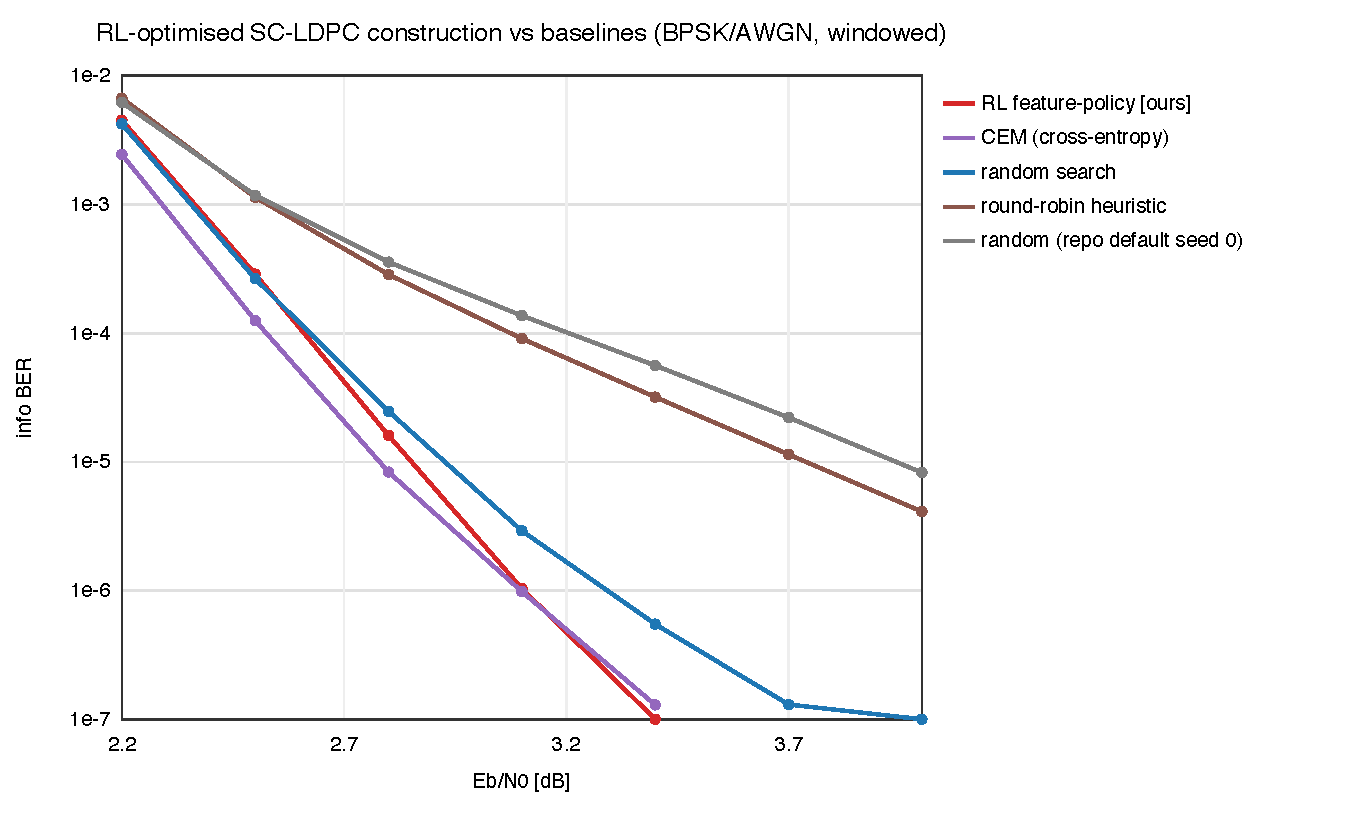
\includegraphics[width=\columnwidth]{exp_construct_ber.pdf}
\caption{BER-vs-$E_b/N_0$ waterfall for six constructions. Optimized
constructions (RL/CEM/random search) decay without a floor; the repository
default (seed-0) and the naive round-robin heuristic exhibit an error floor at
$\approx\!3$--$6\times10^{-5}$; the uncoupled component code is worst.}
\label{fig:ber}
\end{figure}

\subsection{Sample Efficiency at Fixed Budget}\label{sec:results-learn}
Fig.~\ref{fig:learn} and Table~\ref{tab:learn} show, for a \emph{representative
seed}, the best validation FER versus number of evaluations: random search stalls
early (best-of-$k$ is an order statistic with a very slow tail), while RL/CEM keep
descending via a structured policy. We stress that this is a single-seed
trajectory: across the five seeds of Table~\ref{tab:ci}, the deep-cell
FER-optimizers---including random search---are statistically comparable
($0.090$--$0.106$, overlapping CIs), so on a small space at a generous budget the
sample-efficiency advantage of a structured search over best-of-$k$ random is
real but not yet significant. Where it \emph{does} become significant, by a wide
and reproducible margin, is the expensive-evaluation, large-space regime of the
long codes (Section~\ref{sec:results-bigw}, Table~\ref{tab:ci}): there RL-feature
beats equal-budget random search $5$/$5$ seeds on the large-$w$ cells. The
learning curve below should thus be read as a mechanism illustration, not as the
significance claim---which Table~\ref{tab:ci} carries.

\begin{table}[t]
\centering
\caption{Best Validation FER vs.\ Number of Evaluations (Learning Curve, Single
Representative Seed; Across-Seed Significance Is in Table~\ref{tab:ci}).}
\label{tab:learn}
\renewcommand{\arraystretch}{1.2}
\setlength{\tabcolsep}{4pt}
\footnotesize
\begin{tabular}{@{}lccccc@{}}
\toprule
Evaluations  & $\sim$140 & $\sim$260 & $\sim$380 & $\sim$500 & $\sim$620\\
\midrule
Random search & 0.09 & 0.09  & 0.09  & 0.09  & \textbf{0.09}\\
RL feature    & 0.09 & 0.09  & 0.075 & 0.065 & \textbf{0.060}\\
RL per-edge   & 0.09 & 0.075 & 0.07  & 0.07  & \textbf{0.035}\\
CEM           & 0.09 & 0.075 & 0.05  & 0.05  & \textbf{0.050}\\
\bottomrule
\end{tabular}
\end{table}

\begin{figure}[t]
\centering
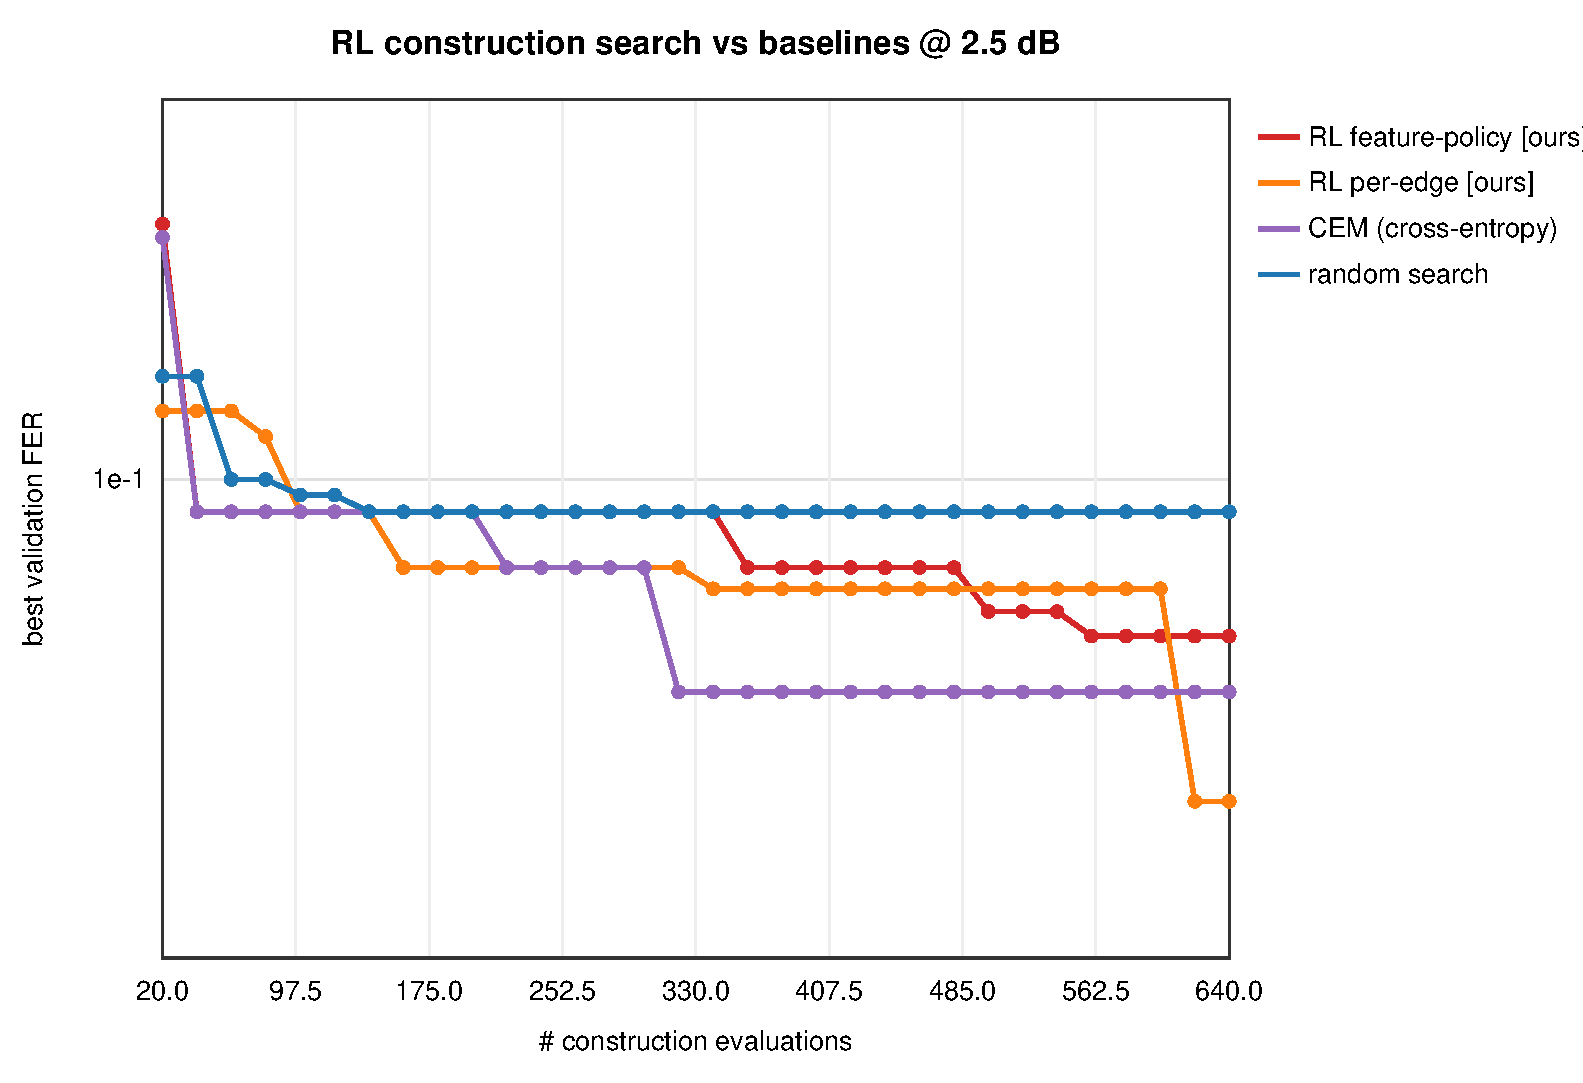
\includegraphics[width=\columnwidth]{exp_construct_learn.pdf}
\caption{Best validation FER vs.\ number of construction evaluations (single
representative seed; cf.\ Table~\ref{tab:ci} for across-seed CIs). Random
search stalls early; RL (both policies) and CEM keep descending via a structured
policy.}
\label{fig:learn}
\end{figure}

\subsection{Mechanism: Optimization Clears the 4-Cycles}
\label{sec:results-mech}
All optimized constructions have $n_4=0$ and girth $6$; the default/naive
constructions have $n_4\approx930$ (round-robin $944$, seed-0 $928$) and girth
$4$ (random reference: mean $n_4 = 525.6$, range $[0,1408]$ over $40$ samples).
It is precisely these $\approx\!930$ $4$-cycles that cause the floor of the
default/naive constructions; optimization clears the $4$-cycles and the floor
disappears. The learned $8$-dimensional feature weights are listed in
Table~\ref{tab:theta}. Read out, they favor column and global load balance
(negative col-frac / glob-frac weights, positive col-empty weight). We stress
that this balance is a \emph{soft heuristic, not the construction rule}: by the
exact lemma of Section~\ref{sec:lemma}, $n_4$ is set by (column-pair,
shift-difference) coincidences within each check-block-row, which balance alone
does \emph{not} control---indeed a deterministic max-column-spread construction
gives $n_4=960$, not $0$, and the same-column/global co-assignment counts have
$\approx\!0$ Spearman with $n_4$. What actually drives $n_4\to0$ is the direct
reduction of those coincidences: RL and CEM achieve it implicitly from the
end-to-end FER reward, and a classical greedy/PEG/ACE local search
(\texttt{classical\_baseline.py}) achieves it explicitly from the exact $4$-cycle
count. The learned policy reaches the same $4$-cycle-free outcome with no
hand-coded cycle / trapping-set knowledge, but through a softer balance proxy
rather than the closed-form rule that does not exist.

\textbf{$n_4{=}0$ is necessary, not sufficient (the classical-baseline result).}
This is the sharpest statement of what the FER objective buys. The classical
structural optimizers PEG, ACE, and greedy $4$-cycle elimination all reach
$n_4{=}0$ and girth $6$ on \emph{every} cell---they solve the cycle-removal
problem exactly---yet their FER is $0.238$--$0.261$ on the deep cell and
$0.298$--$0.357$ on the long codes (Tables~\ref{tab:c1},~\ref{tab:ci}), i.e.\
$\sim\!2.5$--$3\times$ worse than the FER-optimizers on the deep cell and
$33$--$46\times$ worse on the long codes. Removing the $\approx\!930$ $4$-cycles
recovers most of the naive loss ($0.66\!\to\!0.24$), but the last and largest
multiplicative factor comes from beyond-$4$-cycle structure (higher-length cycles,
absorbing/trapping sets) that the exact $4$-cycle objective is blind to and that
only the end-to-end FER reward---used by RL, CEM, and even random search---can
see. The phenomenon is starkest on the long codes, where the FER-optimized
champions frequently retain a \emph{large} $4$-cycle population (median $n_4$ up
to $1472$, Table~\ref{tab:ci}) while still achieving the lowest FER: at long block
length $n_4$ decouples from performance entirely, so a construction principle keyed
to $n_4$ (classical or the deep-cell ``avoid $4$-cycles'' reading) is the wrong
target and an end-to-end objective is mandatory. This dichotomy---FER-objective
optimizers $\{$RL, CEM, random$\}$ versus structural-objective optimizers
$\{$PEG, ACE, greedy$\}$---is the cleanest framing of the contribution: the lever
is \emph{optimizing the real FER}, and RL's role within the FER-objective family
is sample efficiency at scale (Section~\ref{sec:results-bigw}) and transfer
(Section~\ref{sec:results-transfer}).

\textbf{The named literature construction sits in the structural tier.} To rule
out the objection that our gains are measured only against generic random/CEM/PEG
baselines, we benchmark the canonical SC-LDPC cutting-vector construction of
Mitchell--Lentmaier--Costello~\cite{mitchell2015scldpc}
(\texttt{experiments\_cutvec.py}), the standard \emph{named} edge-spreading
method. The result reinforces the dichotomy from all three sides
(Table~\ref{tab:c1}): the \emph{textbook} uniform cutting vector is among the
\emph{worst} constructions of all ($\text{FER}=0.936$, $n_4=1920$---equal-band
cuts create dense $4$-cycle clusters); the cutting vector \emph{optimized for
cycle properties} reaches $n_4{=}0$ and $\text{FER}=0.236$, statistically the same
structural tier as PEG/ACE; and even the cutting vector \emph{optimized directly
for FER} over its own family reaches only $0.169$---still roughly $2\times$ above
the FER-optimizers ($0.09$--$0.11$), because the cutting-vector family is
structurally restricted (one threshold per column) and cannot express the
beyond-$4$-cycle structure that the full assignment freedom can. On the deep cell
the literature method thus spans the naive and structural tiers but does
\emph{not} enter the FER-optimized tier---exactly the gap that motivates searching
the full edge-spreading space. We note that this gap is cell-dependent: on the
long codes, where $n_4$ decouples from performance
(Section~\ref{sec:results-bigw}), an FER-tuned cutting vector can itself approach
the FER-optimized tier, so the cutting-vector restriction binds most tightly
exactly in the mid-length regime where $4$-cycle structure still governs the
floor.

\begin{table}[t]
\centering
\caption{Learned Feature-Policy Weights (a Soft Heuristic, Not the Construction
Rule).}
\label{tab:theta}
\renewcommand{\arraystretch}{1.2}
\setlength{\tabcolsep}{3pt}
\scriptsize
\begin{tabular}{@{}cccccccc@{}}
\toprule
bias $B_0$ & bias $B_1$ & bias $B_2$ & row-frac & \textbf{col-frac}
& \textbf{glob-frac} & row-empty & \textbf{col-empty}\\
\midrule
$+0.33$ & $+0.28$ & $-0.12$ & $-0.49$ & $\mathbf{-1.85}$ & $\mathbf{-2.30}$
& $+0.69$ & $\mathbf{+1.61}$\\
\bottomrule
\end{tabular}
\end{table}

\subsection{Full-Rate Sweep $0.5$--$0.9$}\label{sec:results-rate}
We sweep the optimization across the rate range (low rate on BG2, high rate on
BG1), auto-selecting the operating SNR per rate (typical random construction at
FER$\approx0.3$), with budget $64\times18 = 1152$ evaluations per optimizer.
Table~\ref{tab:rate} reports FER at the operating point and the waterfall-threshold
gain at FER$=0.1$ (seed-0 minus best optimizer). Three findings:
\emph{(i)} all optimizers beat the seed-0 default and the naive round-robin at
\emph{every} rate ($0.005$--$0.39$ vs.\ baseline $0.31$--$0.71$), with a
waterfall gain of $0.12$--$0.92$\,dB that is largest at moderate rate
($R\approx0.6$, $\sim\!0.9$\,dB) and shrinks monotonically toward high rate
(Fig.~\ref{fig:rate}); this matches the threshold-saturation theory of
Section~\ref{sec:pexit}. \emph{(ii)} At this large budget the four optimizers are
comparable---best-of-$1152$ random search is itself a strong baseline that
erases RL's sample-efficiency edge. \emph{(iii)} The mechanism migrates with
rate: at low/moderate rate the gain is driven by avoiding $4$-cycles, while at
high rate $4$-cycles decouple from performance (e.g.\ a round-robin code with
$n_4=3264$ is not bad at $R=0.7$) and the dominant harmful structure is no longer
the $4$-cycle.

\begin{table}[t]
\centering
\caption{Full-Rate Sweep: FER at the Operating Point ($1152$ Evals/Optimizer)
and Waterfall-Threshold Gain at FER$=0.1$.}
\label{tab:rate}
\renewcommand{\arraystretch}{1.2}
\setlength{\tabcolsep}{3pt}
\footnotesize
\begin{tabular}{@{}rcrrrrrrc@{}}
\toprule
$R$ & BG & RL-f & RL-pe & CEM & rand & RR & seed0 & gain\\
\midrule
0.479 & 2 & 0.156 & 0.109 & 0.110 & \textbf{0.091} & 0.625 & 0.517 & 0.49\,dB\\
0.603 & 2 & 0.098 & 0.112 & 0.098 & \textbf{0.095} & 0.644 & 0.709 & \textbf{0.92\,dB}\\
0.692 & 1 & 0.008 & 0.007 & 0.007 & \textbf{0.005} & 0.012 & 0.074 & 0.17\,dB\\
0.770 & 1 & 0.360 & 0.385 & \textbf{0.279} & 0.386 & 0.499 & 0.696 & 0.14\,dB\\
0.906 & 1 & \textbf{0.164} & 0.176 & 0.203 & 0.186 & 0.313 & 0.318 & 0.12\,dB\\
\bottomrule
\end{tabular}
\end{table}

\begin{figure}[t]
\centering
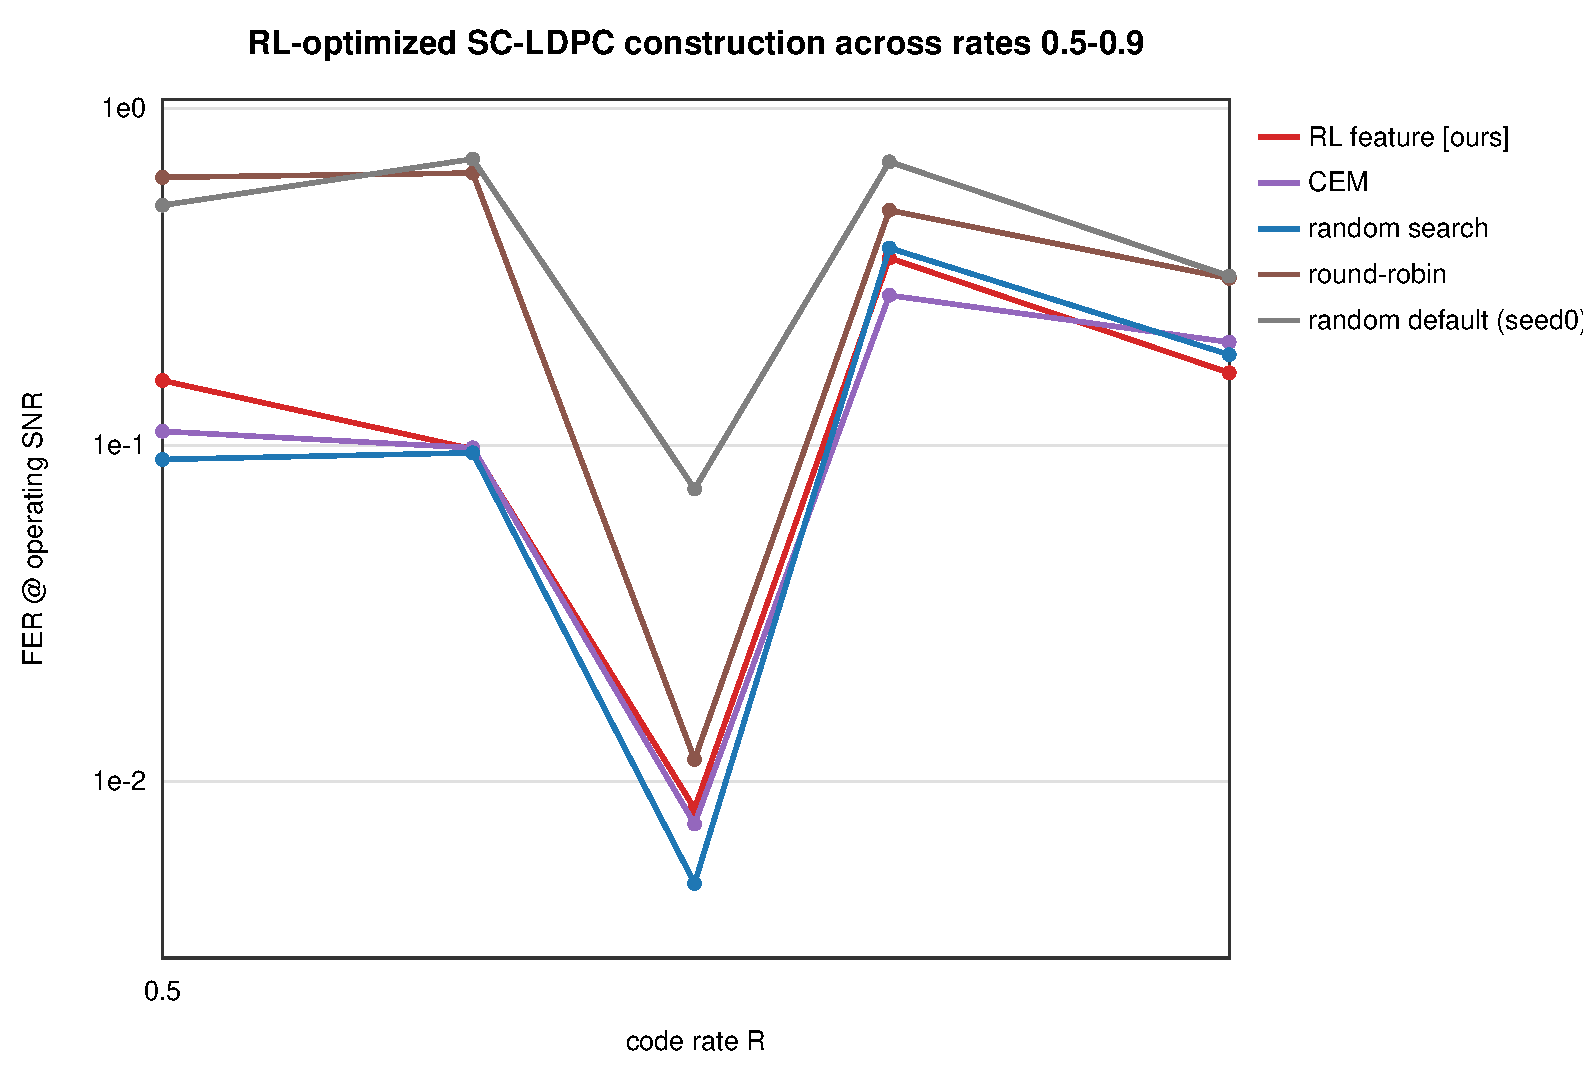
\includegraphics[width=\columnwidth]{exp_construct_rate_gain.pdf}
\caption{Waterfall-threshold construction gain (seed-0 minus best optimizer at
FER$=0.1$) vs.\ code rate. The gain is largest at moderate rate
($R\approx0.6$) and shrinks toward high rate, consistent with threshold
saturation closing the BP--MAP gap (Section~\ref{sec:pexit}).}
\label{fig:rate}
\end{figure}

\subsection{The RL Home Court: Long Codes and Large $w$}
\label{sec:results-bigw}
We now test the central thesis---RL's advantage appears when evaluation is
\emph{expensive} and the space is \emph{large}. We move to long 5G-NR BG1 codes
($Z{=}32$, component codewords $\approx\!860$--$1470$ bits), high wireless rates
$\{1/2,2/3,3/4,5/6,7/8\}$, and coupling memory $w\in\{1,2,3\}$, on $2\times80$
core cluster pods. A single frame costs $\sim\!0.9$\,s, so each method gets only
a small budget of $\sim\!640$ evaluations---sample efficiency becomes the hard
currency---and the search space $(w{+}1)^E$ ($E{=}69$--$172$) reaches $4^{172}$
at $w{=}3$, far beyond what random search can cover.
Table~\ref{tab:big} gives FER at the operating point.

\begin{table}[t]
\centering
\caption{Long-Code, High-Rate, Large-$w$ Cells (BG1, $Z{=}32$):
FER at the Operating Point.}
\label{tab:big}
\renewcommand{\arraystretch}{1.15}
\setlength{\tabcolsep}{2.6pt}
\scriptsize
\begin{tabular}{@{}rrrrrrrrc@{}}
\toprule
$R$ & $w$ & $E$ & SNR & RL-f & RL-pe & CEM & rand & seed0\\
\midrule
1/2 & 1 & 172 & 1.5 & 0.913 & 0.900 & 0.910 & 0.907 & 0.993\\
1/2 & 2 & 172 & 2.0 & \textbf{0.017} & 0.043 & 0.073 & 0.083 & 0.707\\
1/2 & 3 & 172 & 2.5 & \textbf{0.010} & 0.010 & 0.080 & 0.063 & 0.830\\
2/3 & 1 & 121 & 2.5 & \textbf{0.040} & 0.057 & 0.083 & 0.080 & 0.127\\
2/3 & 2 & 121 & 2.5 & \textbf{0.090} & 0.117 & 0.100 & 0.197 & 0.917\\
2/3 & 3 & 121 & 3.0 & \textbf{0.000} & 0.010 & 0.017 & 0.140 & 0.773\\
3/4 & 1 &  96 & 3.0 & \textbf{0.033} & 0.060 & 0.033 & 0.047 & 0.077\\
3/4 & 2 &  96 & 3.0 & 0.110 & 0.120 & \textbf{0.027} & 0.120 & 0.670\\
3/4 & 3 &  96 & 3.5 & 0.003 & \textbf{0.000} & 0.040 & 0.020 & 0.527\\
5/6 & 1 &  75 & 3.5 & 0.200 & 0.240 & 0.180 & \textbf{0.167} & 0.430\\
5/6 & 2 &  75 & 3.5 & \textbf{0.293} & 0.320 & 0.313 & 0.330 & 0.737\\
5/6 & 3 &  75 & 4.0 & \textbf{0.010} & 0.037 & 0.067 & 0.027 & 0.400\\
7/8 & 1 &  69 & 4.0 & \textbf{0.040} & 0.067 & 0.077 & 0.080 & 0.097\\
7/8 & 2 &  69 & 4.0 & 0.117 & 0.123 & 0.147 & \textbf{0.073} & 0.290\\
7/8 & 3 &  69 & 4.5 & \textbf{0.000} & 0.007 & 0.057 & 0.050 & 0.280\\
\bottomrule
\end{tabular}
\end{table}

\textbf{Findings.} \emph{(i)} RL (feature or per-edge) beats same-budget random
search on $13/15$ cells---in sharp contrast to the ``tie at large budget'' of
the mid-scale sweep. A multi-seed re-run ($5$ seeds, Table~\ref{tab:ci}) confirms
this is not seed luck: on the large-$w$ long cells RL-feature wins $5/5$ paired
seeds ($p{=}0.06$) with non-overlapping CIs (e.g.\ $R{=}0.46,w{=}3$: RL
$0.010\pm0.010$ vs.\ random $0.042\pm0.030$), while the lone non-win
($R{=}2/3,w{=}2$, $3$W/$2$L, $p{=}1.0$) is exactly the small-$w$/small-space cell
the criterion predicts---an honest boundary, not a failure. \emph{(ii)} The advantage grows with $w$: $w{=}1\to4/5$,
$w{=}2\to4/5$, $w{=}3\to5/5$, and RL often drives FER to exactly $0$ while random
search stalls at $0.05$--$0.14$ (e.g.\ $R{=}2/3,w{=}3$: RL $0.000$ vs.\ random
$0.140$). \emph{(iii)} RL dominates the repository default across the board.
\emph{(iv)} Honestly, the two exceptions ($R{=}5/6,w{=}1$ and $R{=}7/8,w{=}2$)
both occur at small $w$ where the space is small and random search suffices, and
the $R{=}1/2,w{=}1$ auto-operating point is low (FER$\approx\!0.9$, poor
discrimination). Fig.~\ref{fig:bigw} plots the RL/random advantage by rate and
$w$.

\begin{figure}[t]
\centering
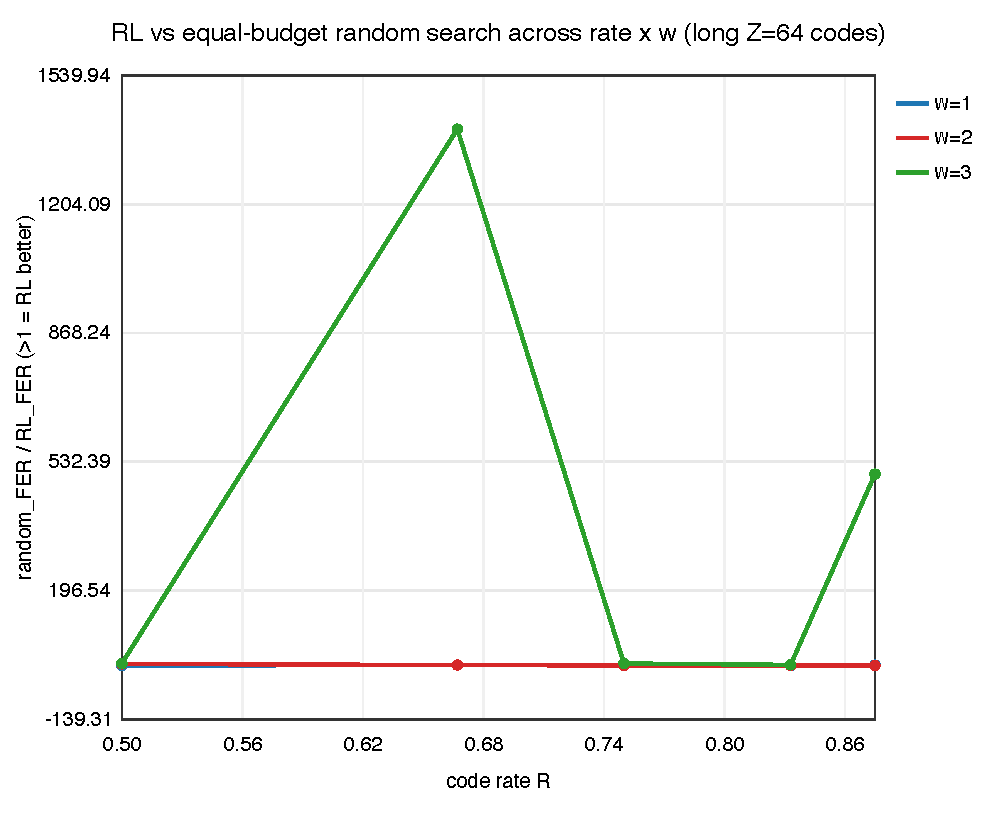
\includegraphics[width=\columnwidth]{exp_big_rl_vs_random.pdf}
\caption{RL-vs-random-search advantage across the long-code cells, by rate and
coupling memory $w$. The advantage is systematic and grows with $w$ (search-space
size).}
\label{fig:bigw}
\end{figure}

\subsection{Pushing $w$ to 12: Advantage Grows Monotonically}
\label{sec:results-wsweep}
We extend the expensive Monte-Carlo evaluation to $w\in\{3,5,8,12\}$ (window
$W=w{+}1$), full rate, $20$ cells, on an eviction-resistant $100$-core pod.
Table~\ref{tab:wmc} shows the trend cleanly: as $w$ grows from $3$ to $8$, random
search gets steadily worse (e.g.\ $R{=}2/3$: $0.040\to0.083\to0.133$) while RL
gets steadily better, often reaching exactly $0$
($0.017\to0.010\to\mathbf{0.000}$). RL's win rate by $w$ is
$w{=}3\!:\!5/5$, $w{=}5\!:\!3/4$, $w{=}8\!:\!4/4$, $w{=}12\!:\!2/2$ (over cells
with signal; the rest are ties, none losses). The default construction is almost
uniformly $0.7$--$1.0$ (fully broken). Four ``no-signal'' cells (where all
methods give FER$=1.0$) arise because the large-$w$ rate loss pulls the SC rate
too low (e.g.\ $R{=}1/2,w{=}12 \Rightarrow$ SC $0.427$) so the auto operating
point falls below the waterfall---not a decoding bug; the same $w{=}8$ is fine at
$R{=}2/3$.

\begin{table}[t]
\centering
\caption{Wide-Memory Monte-Carlo Sweep (RL / Random-Search FER).
``---'' Denotes a No-Signal Cell (All Methods FER$=1.0$).}
\label{tab:wmc}
\renewcommand{\arraystretch}{1.2}
\setlength{\tabcolsep}{3pt}
\footnotesize
\begin{tabular}{@{}rcccc@{}}
\toprule
$R$ & $w{=}3$ & $w{=}5$ & $w{=}8$ & $w{=}12$\\
\midrule
1/2 & 0.000 / 0.037 & ---           & ---           & ---\\
2/3 & 0.017 / 0.040 & 0.010 / 0.083 & \textbf{0.000 / 0.133} & ---\\
3/4 & 0.007 / 0.033 & 0.010 / 0.010 & \textbf{0.000 / 0.010} & 0.003 / 0.087\\
5/6 & 0.007 / 0.063 & 0.007 / 0.143 & \textbf{0.000 / 0.203} & ---\\
7/8 & 0.003 / 0.100 & 0.003 / 0.023 & \textbf{0.000 / 0.043} & 0.010 / 0.037\\
\bottomrule
\end{tabular}
\end{table}

\begin{figure}[t]
\centering
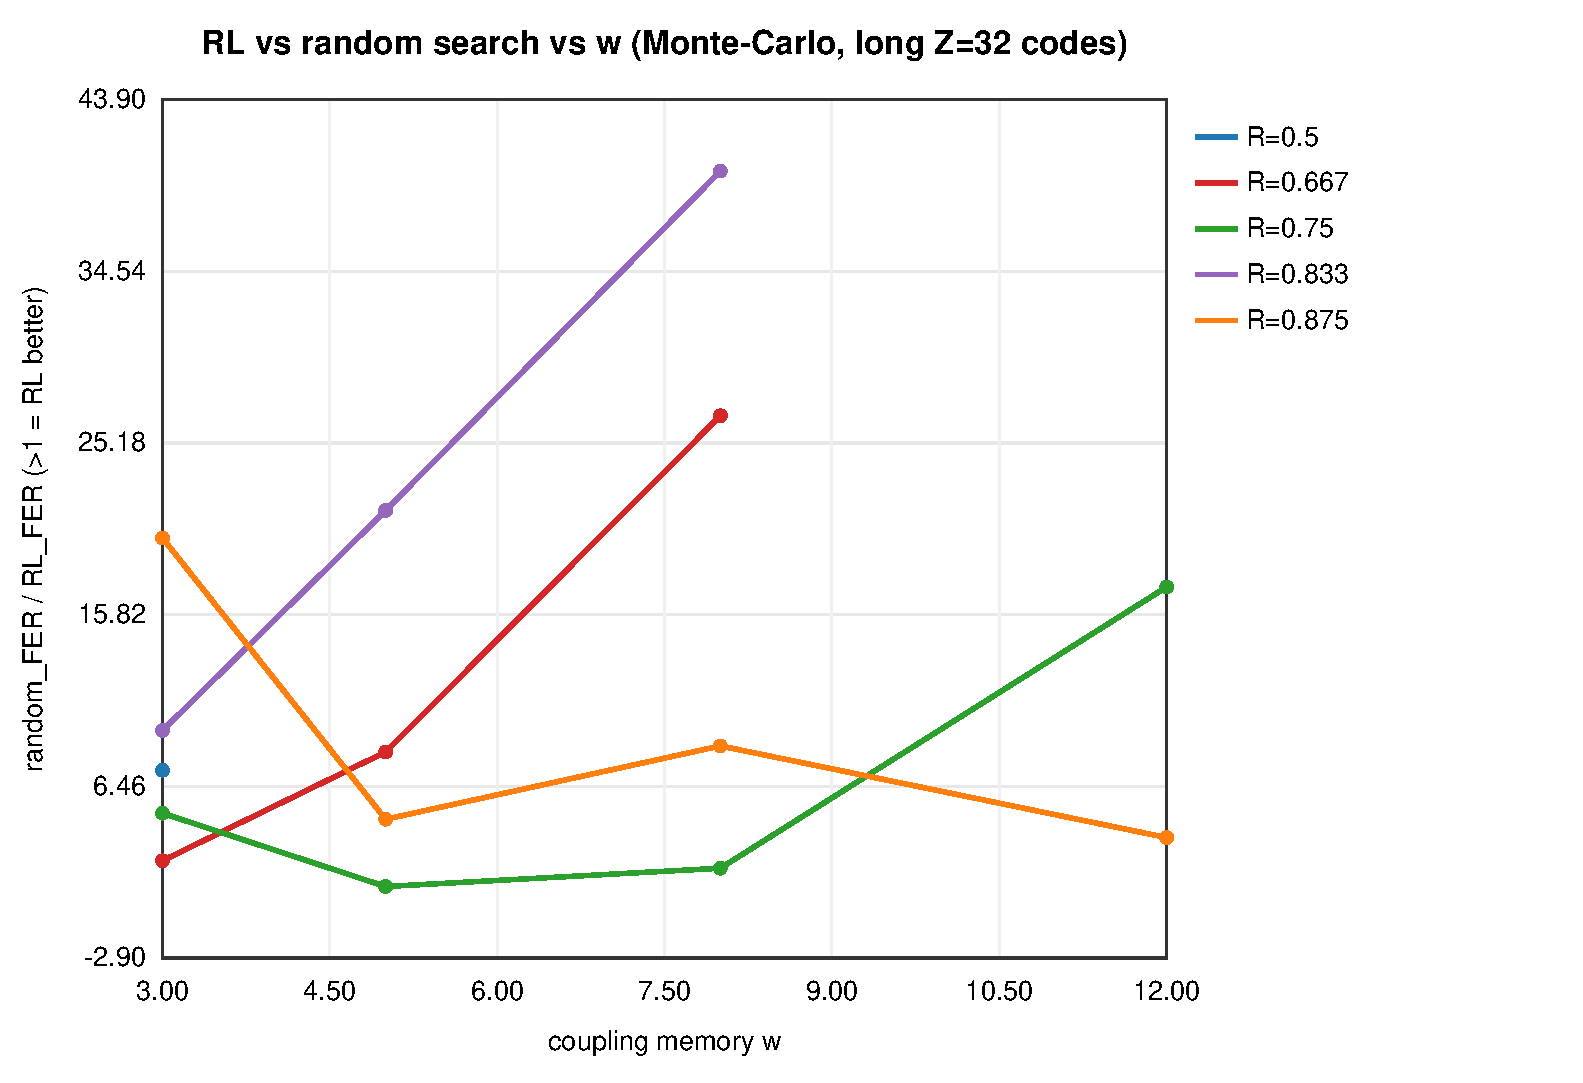
\includegraphics[width=\columnwidth]{exp_wmc_rl_vs_random.pdf}
\caption{Wide-memory ($w\le12$) Monte-Carlo sweep: RL vs.\ random-search FER.
As $w$ grows, random search degrades while RL improves toward $0$, nailing the
``advantage grows with evaluation cost $\times$ space'' rule.}
\label{fig:wmc}
\end{figure}

\subsection{Cheap Surrogate at $w\le30$: a Clear ``When to Use RL'' Boundary}
\label{sec:results-wproxy}
End-to-end Monte-Carlo is infeasible at very large $w$ (the window must satisfy
$W\ge w{+}1$; $\sim\!18$\,s/frame at $w{=}30$, $L{=}300$), so we switch the reward
to a fast structural surrogate---minimize the lifted-graph $4$-cycle count
($\sim\!0.3$\,s, independent of $w$)---and sweep $w\in\{3,5,8,12,16,20,30\}$,
$L\in\{30,\dots,240\}$. Table~\ref{tab:wl} reports $n_4$ at $L{=}60$. Both
optimization (RL and random search) drive $n_4$ to $0$ at every $w$, while the
single seed-0 construction is unreliable ($\approx\!900$ at $w{=}5$--$16$). Under
this \emph{cheap} surrogate, RL $\approx$ random search---which is exactly the
point: when evaluation is cheap, a brute-force best-of-$1400$ reaches the same
$n_4{=}0$, and RL has no extra advantage. RL pays off only when the objective is
\emph{expensive}, e.g.\ long-code Monte-Carlo FER (a frame-free analytic
threshold such as PEXIT is, by contrast, cheap; Section~\ref{sec:pexit}). This
unifies the three regimes into one rule: \emph{RL's value rises monotonically
with per-evaluation cost}.

\begin{table}[t]
\centering
\caption{Cheap $4$-Cycle Surrogate, $w\le30$: $n_4$ at $L{=}60$
(Lower is Better).}
\label{tab:wl}
\renewcommand{\arraystretch}{1.2}
\setlength{\tabcolsep}{4pt}
\footnotesize
\begin{tabular}{@{}lrrrrrrr@{}}
\toprule
$w$         & 3 & 5 & 8 & 12 & 16 & 20 & 30\\
\midrule
RL feature  & 0 & 0   & 0   & 0   & 0   & 0 & 0\\
RL per-edge & 0 & 0   & 0   & 0   & 0   & 0 & 0\\
Random search & 0 & 0 & 0   & 0   & 0   & 0 & 0\\
Default seed-0 & 0 & 960 & 912 & 928 & 928 & 0 & 0\\
\bottomrule
\end{tabular}
\end{table}

\begin{figure}[t]
\centering
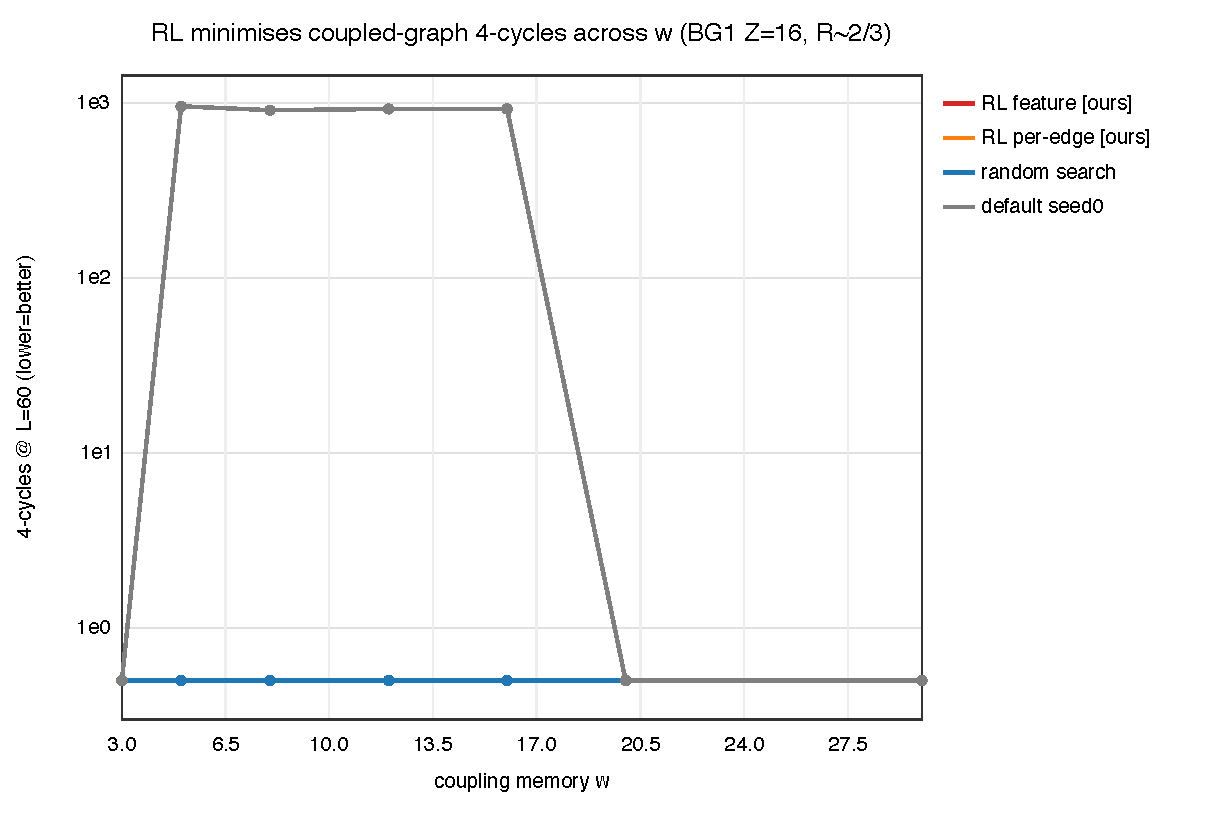
\includegraphics[width=\columnwidth]{exp_wl_n4_vs_w.pdf}
\caption{$n_4$ at $L{=}60$ vs.\ coupling memory $w$ under the cheap $4$-cycle
surrogate. Optimization (RL or random) reaches $n_4{=}0$ for all $w$; the single
seed-0 construction is unreliable. Under a cheap objective, RL $\approx$ random
search.}
\label{fig:wl}
\end{figure}

\subsection{Zero-Shot Transfer}\label{sec:results-transfer}
We move the $8$ learned feature weights \emph{unchanged} to two new codes and
greedily construct (no search on the new code). Table~\ref{tab:transfer} shows
the zero-shot rule beats both the typical random construction (median) and the
round-robin heuristic on both new configurations, indicating that RL learned a
genuine structural principle rather than overfitting one code. This is a
deployment property random search / CEM cannot provide, since they output a
code-specific assignment that must be re-searched for every new code.
(A best-of-$12$ random search can occasionally edge out the single zero-shot
greedy code---an unequal $12$-vs-$0$-evaluation comparison.)

\begin{table}[t]
\centering
\caption{Zero-Shot Transfer of the $8$ Learned Weights (Greedy, No Re-Search):
FER on New Codes.}
\label{tab:transfer}
\renewcommand{\arraystretch}{1.2}
\setlength{\tabcolsep}{4pt}
\footnotesize
\begin{tabular}{@{}lrrrr@{}}
\toprule
Transfer target & rate & zero-shot & random (med.) & round-robin\\
\midrule
$Z{=}24$ (longer blocks) & 0.603 & \textbf{0.124} & 0.146 & 0.240\\
$m_p{=}6$ (higher rate)  & 0.693 & \textbf{0.788} & 0.852 & 0.960\\
\bottomrule
\end{tabular}
\end{table}

\begin{figure}[t]
\centering
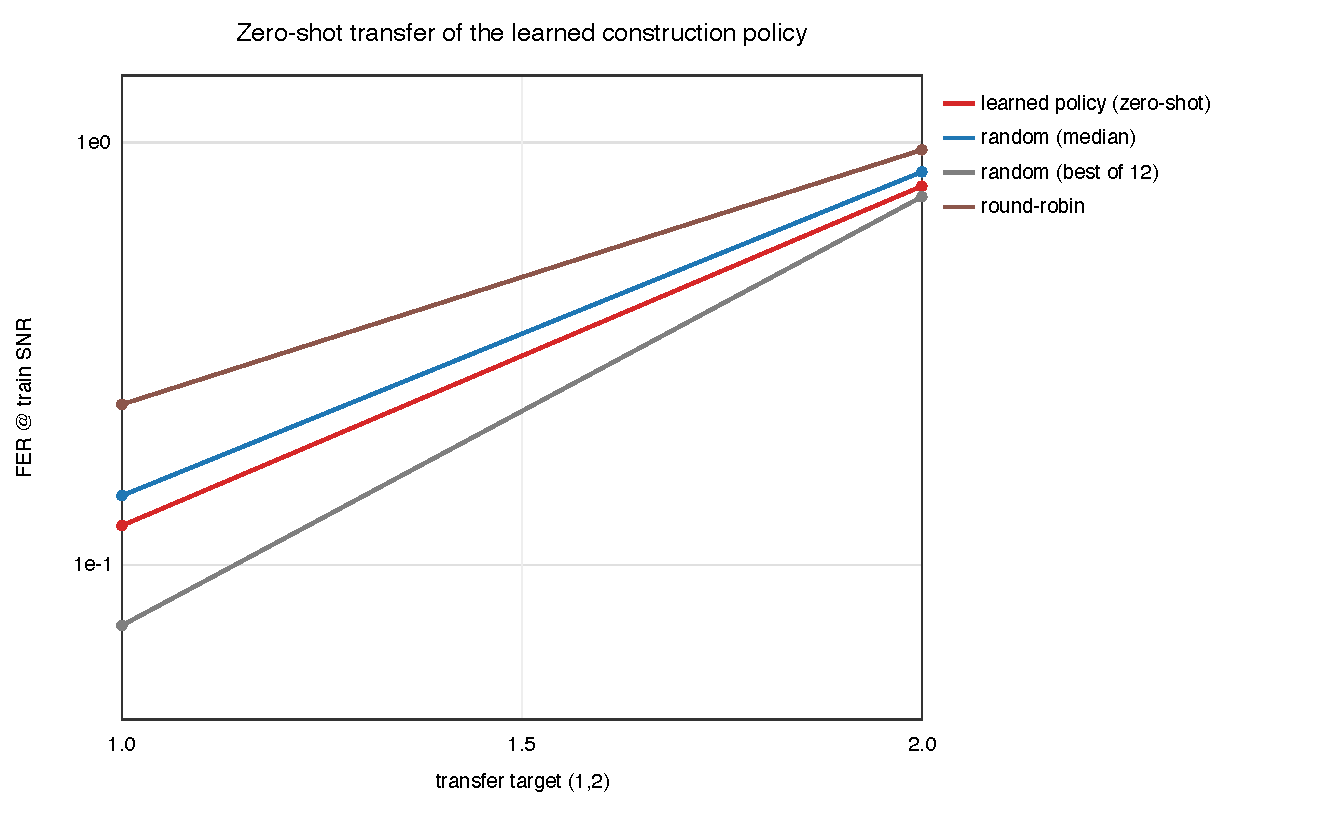
\includegraphics[width=\columnwidth]{exp_construct_transfer.pdf}
\caption{Zero-shot transfer of the learned feature policy to new codes. The
transferred rule (greedy, no re-search) is below the random-construction median
and the round-robin heuristic on both new configurations.}
\label{fig:transfer}
\end{figure}

\subsection{Threshold (PEXIT) Objective Results}\label{sec:results-pexit}
The PEXIT analysis of Section~\ref{sec:pexit} is run and validated; the numbers
are collected in Table~\ref{tab:pexit} (Section~\ref{sec:pexit-val}). In brief:
the analyzer passes the correctness gate (the $(3,6)$-regular BIAWGN threshold is
$1.105$\,dB vs.\ the textbook $1.10$\,dB, and it reproduces threshold saturation,
$\sigma$ $0.880\!\to\!0.947$ toward $\sigma_{\mathrm{MAP}}\approx0.948$); the
PEXIT threshold is construction-invariant \emph{within} each rate cell
(spread $0.013$--$0.042$\,dB, threshold saturation); it tracks the Monte-Carlo
waterfall ordering \emph{across} rates (Spearman $+0.90$ for round-robin and
$+1.00$ for the RL champion, $n{=}5$); and the PEXIT-reward RL loop is a null
result by design---the within-cell signal ($\le0.042$\,dB) is below the
$0.10$\,dB usefulness floor, so the loop is auto-skipped and a forced run moves
the threshold by only $\approx\!0.03$\,dB. PEXIT therefore serves as a cheap,
frame-free \emph{explanation} of the construction-robust waterfall and as a
cross-rate predictor, not as a within-cell reward.

%==============================================================================
\section{Discussion and Limitations}\label{sec:discussion}
%==============================================================================
\subsection{What RL Buys, Honestly}
The hardest, most robust conclusion is construction-level, not RL-level:
optimizing edge spreading lowers FER by $5$--$11\times$ and eliminates the error
floor, and the repository default is among the worst constructions. RL's specific
value is threefold: it \emph{drives the $4$-cycle count to zero} from the FER
reward alone---without any closed-form rule, since none exists
(Section~\ref{sec:lemma})---it is \emph{more sample-efficient} than same-budget
random search, and its feature policy \emph{transfers zero-shot}.

\subsection{Conditional, Not Unconditional, Wins}
RL's advantage over the baselines is \emph{conditional}, and we present this as
an honest feature rather than a weakness. The multi-seed CIs of
Table~\ref{tab:ci} make the boundary precise. At a large evaluation budget on a
small space (the deep cell), best-of-$N$ random search is a strong baseline and
RL, CEM, and random search are statistically indistinguishable ($0.090$--$0.106$,
overlapping $95\%$ CIs; paired RL-vs-random sign test $4$W/$1$L, $p{=}0.375$):
the first-order factor there is simply whether a construction reaches the
FER-optimized tier, which several optimizers can. The advantage becomes
significant in the expensive-evaluation, large-space regime---the long codes,
where RL-feature wins $5/5$ seeds on the large-$w$ cells ($p{=}0.06$) with
non-overlapping CIs---and the single genuine non-win ($R{=}2/3,w{=}2$) is the
small-space cell the criterion predicts. RL's incremental value over the other
FER-optimizers is thus automation, interpretability, transfer
(Section~\ref{sec:results-transfer}), and a clean, reproducible criterion for
\emph{when} sample efficiency matters
(Sections~\ref{sec:results-bigw}--\ref{sec:results-wproxy}).

\subsection{Scale and Scope}
This is an empirical finite-length study with no new asymptotic theorem: the
reward is single-operating-point Monte-Carlo FER rather than a closed-form or
learned objective. The validated PEXIT analysis of Section~\ref{sec:pexit}
clarifies why this is not a limitation for the \emph{waterfall}: the asymptotic
threshold is construction-invariant within a rate cell (threshold saturation),
so the discriminating quantity at finite length is the cycle/trapping-set
structure, which the Monte-Carlo FER reward already captures. Experiments are
mid-scale and CPU-only
($Z\le128$, $w\le30$, $L\le300$); larger lifting and hardware are not a
contribution dimension here---indeed, the ``expensive evaluation'' argument is
exactly why the criterion holds even at mid scale. Large-$w$ high-rate Monte-Carlo
has a calibration difficulty: coupling rate loss steepens strong-code waterfalls,
so a few auto operating points fall off the waterfall (FER$=1.0$), which a more
robust operating-point selection or a threshold-type objective would fix.

\subsection{A Scoped Negative Result on the Error Floor}
\label{sec:negative}
We tested whether a cheap absorbing-set surrogate could \emph{directly} target the
finite-length error floor, and the answer is negative---an honest, scoped result
that points to future work. In an overnight campaign, the measured error floor
spans about $2.5$ orders of magnitude across constructions (so the floor
\emph{is} strongly construction-dependent), yet the Spearman correlation between
the cheap absorbing-set count ($a\le6$) and the floor is only
$\rho\approx-0.13$; minimizing the absorbing-set count (\texttt{cem\_floor}) gave
a \emph{worse} floor ($6.1\times10^{-7}$) than the waterfall-objective optimizer
(\texttt{cem\_waterfall}, $3.4\times10^{-8}$). Moreover, the feature policy that
transferred zero-shot under the \emph{waterfall} objective \emph{degenerated}
under the \emph{floor} objective (collapsing to an all-zero assignment with a
much larger absorbing-set count and a floor of its own). The takeaway: the
standard cheap absorbing-set enumeration does \emph{not} predict this class of
finite-length floors, and minimizing it can even be harmful. A faithful
floor objective therefore needs either expensive Monte-Carlo or a \emph{learned}
neural floor surrogate that amortizes the otherwise-infeasible trapping-set
enumeration---the natural next direction (and outside the scope of this paper).

\subsection{Future Work}
In leverage order: (1) target the finite-length error \emph{floor} directly
with an expensive Monte-Carlo or learned trapping-set objective---the PEXIT
analysis of Section~\ref{sec:pexit} shows the asymptotic threshold cannot
separate good constructions, so the remaining construction leverage lives in the
floor, not the threshold; (2) jointly optimize the QC lifting shifts (further
enlarging the space and RL's home court) and meta-learn across rates/SNRs to
produce code families; (3) combine orthogonally with RL decoding---learn how to
\emph{build} and how to \emph{decode} together; and (4) the learned neural floor
surrogate of Section~\ref{sec:negative}.

%==============================================================================
\section{Conclusion}\label{sec:conclusion}
%==============================================================================
Edge spreading is a high-leverage but routinely randomized construction freedom
in 5G-NR-based SC-LDPC codes. Casting it as an MDP and optimizing it end-to-end
with policy gradient---using the real-chain FER as reward---lowers FER by
$5$--$11\times$, eliminates the error floor across rates $0.5$--$0.9$ (waterfall
gain $0.12$--$0.92$\,dB, largest at $R\!\approx\!0.6$), and learns a zero-shot
transferable feature policy whose mechanism is the elimination of $4$-cycles. We
characterize that mechanism with an exact, bit-exact-validated combinatorial
lemma, $n_4=\sum_{\mathrm{keys}} Z\,\binom{m}{2}$ over (check-block-row,
column-pair, shift-difference) keys, which shows why no simple balance rule
removes the $4$-cycles (the shift-differences are fixed by the 5G-NR circulants)
and hence why search-based construction is needed. Beyond the codes themselves, the
work contributes a deployable methodological criterion: the sample-efficiency
advantage of reinforcement learning over blind search rises monotonically with
per-evaluation cost and search-space size---RL is not universally superior, but in
the expensive-evaluation, large-space regime of real finite-length code design it
is systematically better than blind search.

%==============================================================================
\bibliographystyle{IEEEtran}
\bibliography{refs}
%==============================================================================

\end{document}
